\chapter{Game 15}

\begin{figure}[H]
   \centering
   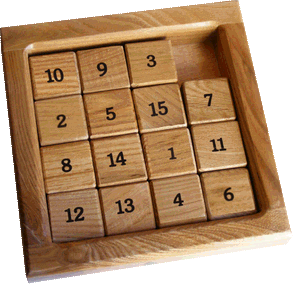
\includegraphics[width=1.0\linewidth,height=0.5\linewidth]{fig060001.png}
   \caption{"The 15 Game" \\ http://www.murderousmaths.co.uk/games/loyd/15 puzzle wood.gif}
\label{fig060001}
\end{figure}

"Game 15" (Fig. \ref{fig060001}) is a children's puzzle from the "graph journey" group of games. The playing field is formed in 4x4 cells, and it contains 15 tiles. The tiles are numbered and the sixteenth position is empty. The empty position serves as a buffer into which adjacent tiles can be moved. Using the buffer cell, the game is shuffled and the goal is to arrange the tiles according to the starting numbering.

\section{Structuring the GUI}

This is a children's game, the arrangement of which is not particularly difficult, and only the last row of the puzzle creates complexity. The relatively simple organization of the game makes it ideal for implementation as an App Inventor application. With the help of only 16 buttons, the entire necessary interface can be built. Crafting begins with the creation of a new project (Fig. \ref{fig060002}).

\begin{figure}[H]
   \centering
   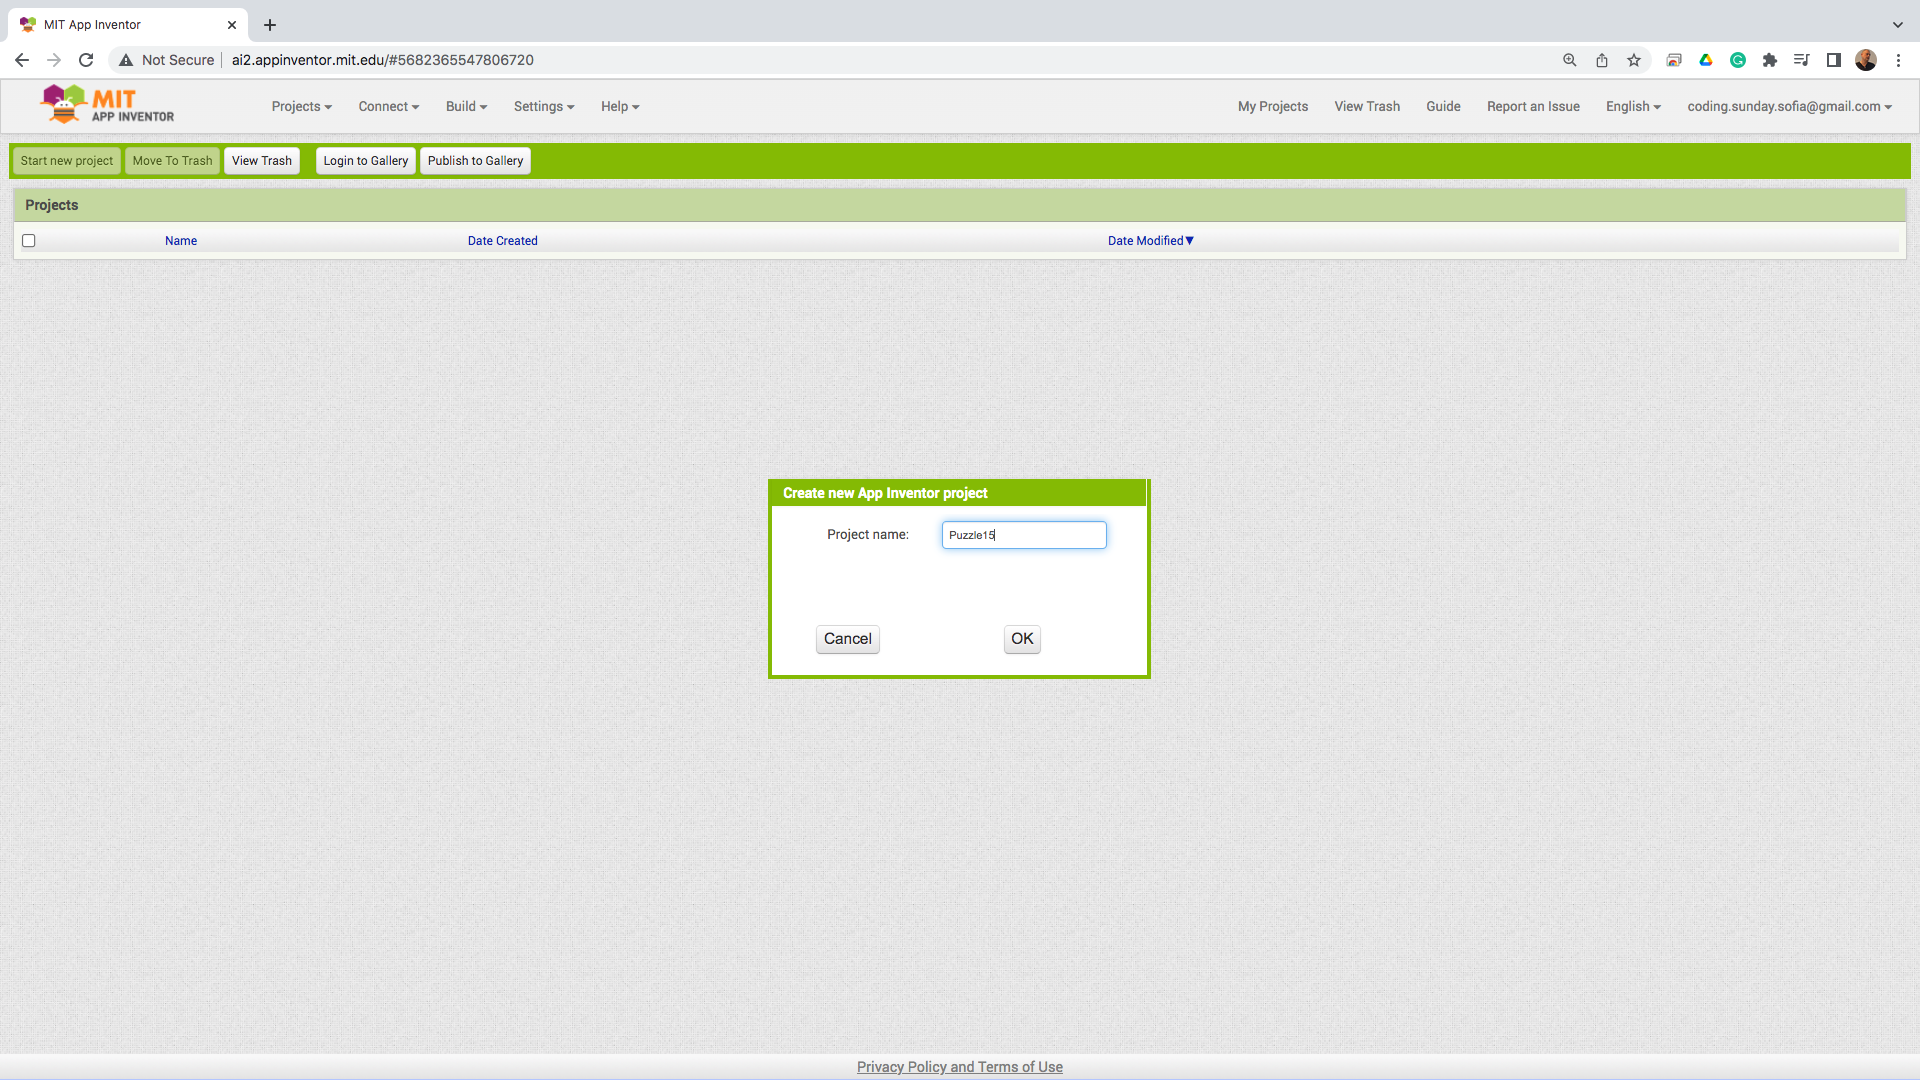
\includegraphics[width=1.0\linewidth,height=0.5\linewidth]{fig060002.png}
   \caption{Starting a new project for "The Game 15"}
\label{fig060002}
\end{figure}

Since 15 numbered buttons and one unnumbered button will be used, it is best to organize them with a table-type layout manager, with 4 rows and 4 columns (Fig. \ref{fig060003}).

\begin{figure}[H]
   \centering
   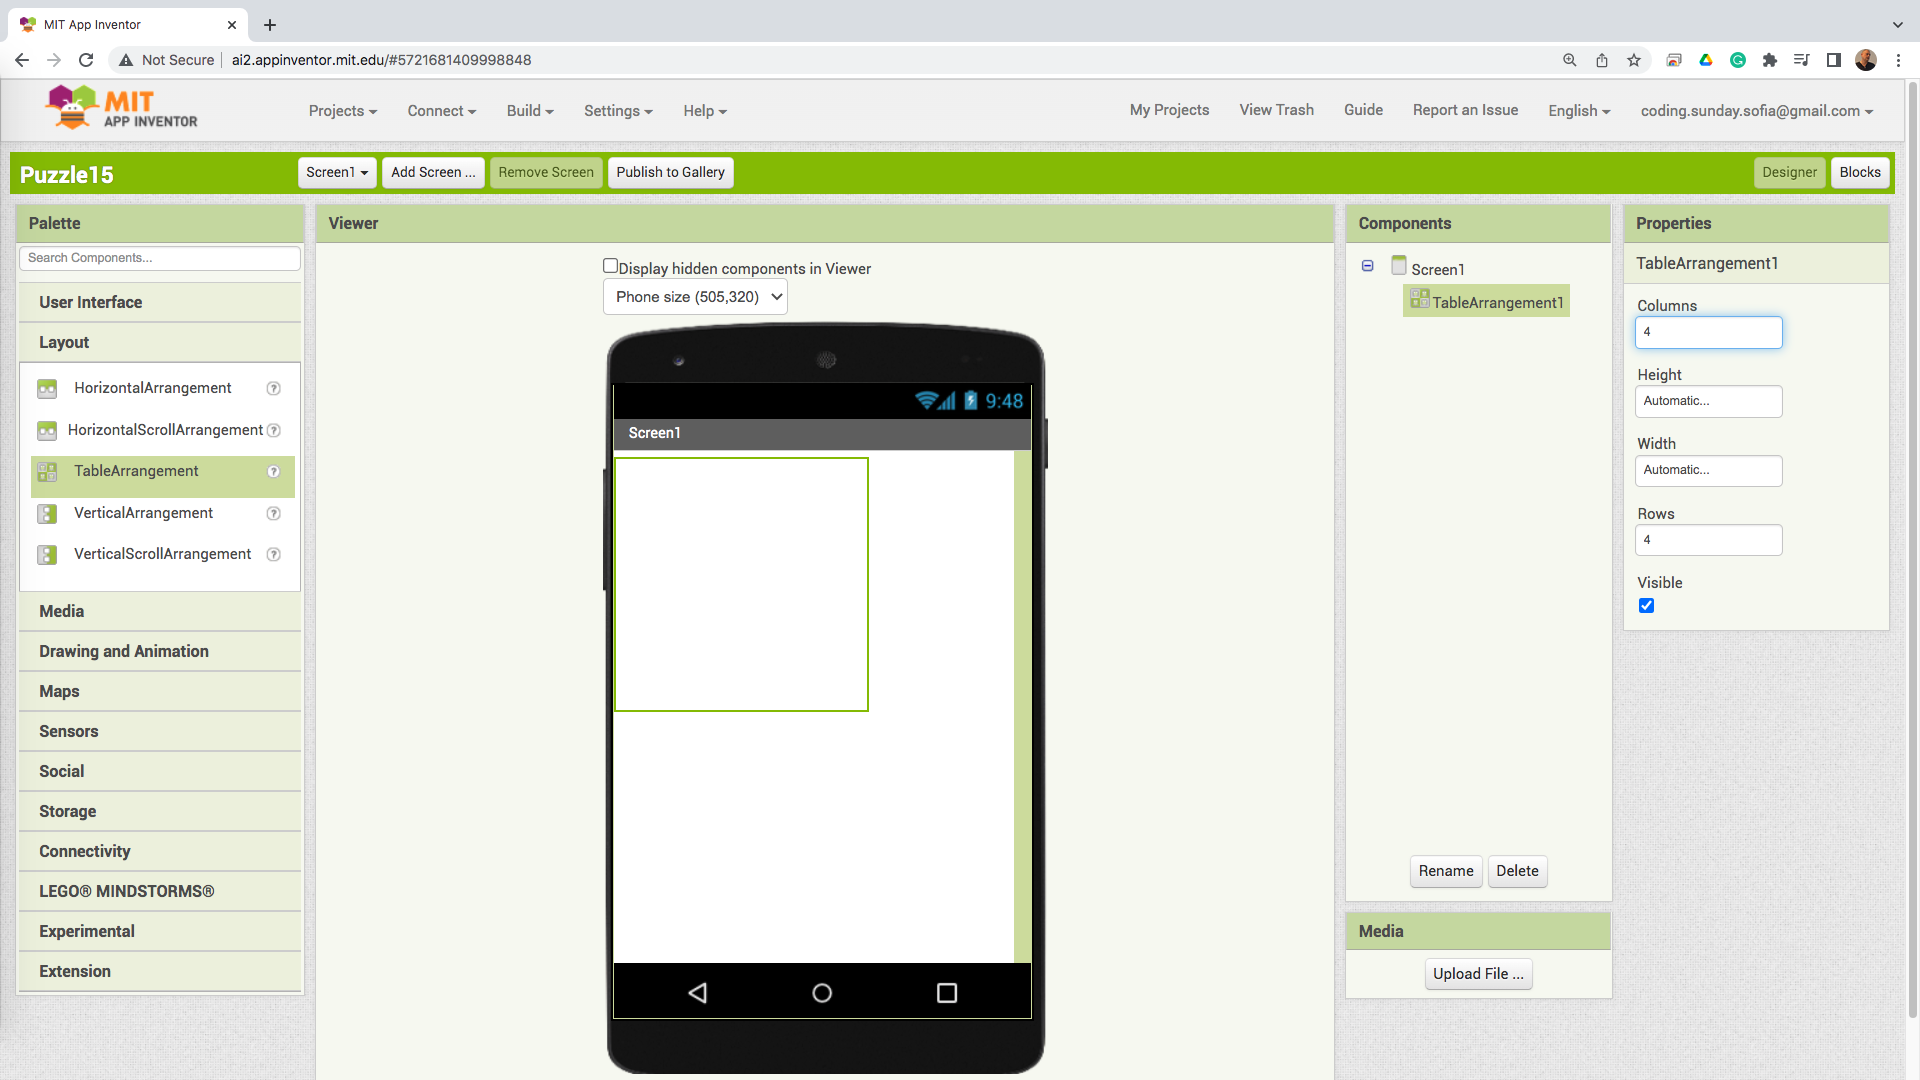
\includegraphics[width=1.0\linewidth,height=0.5\linewidth]{fig060003.png}
   \caption{4x4 cell content manager}
\label{fig060003}
\end{figure}

Then 16 buttons are placed (Fig. \ref{fig060004}), with the odd numbers colored red and the even numbers blue. Coloring enhances the visual effect of the game. The sixteenth button instead of a label has two blank spaces so that its width matches the width of the other buttons. Without additional settings, the width of the buttons is determined by the number of characters in their labels.

\begin{figure}[H]
   \centering
   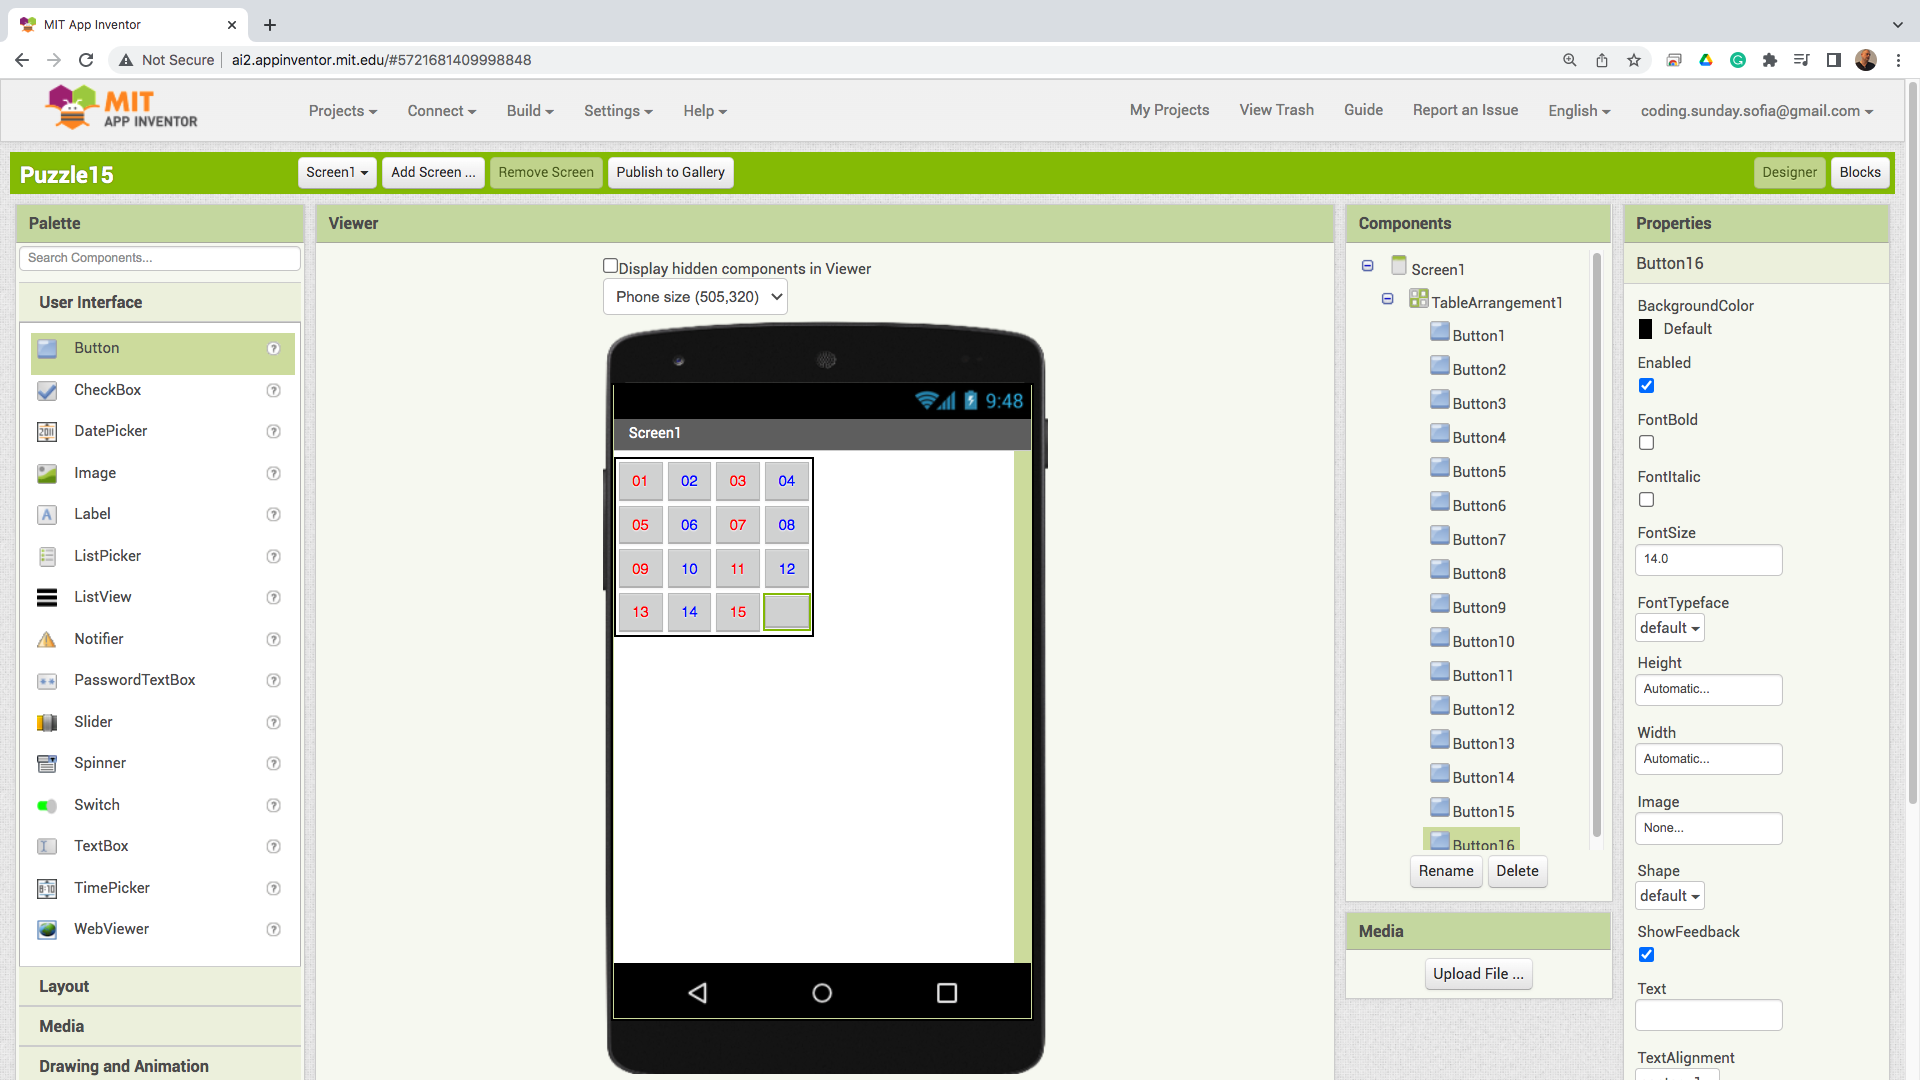
\includegraphics[width=1.0\linewidth,height=0.5\linewidth]{fig060004.png}
   \caption{Placement of 16 buttons}
\label{fig060004}
\end{figure}

It is possible to swap the buttons themselves when a button adjacent to the empty cell is pressed, but it is much easier to swap the labels and colors of the buttons and have the buttons themselves always stay in their original places. The button press will be caught in a common event for all buttons, but after the press it must be determined if the empty cell is adjacent. The most elegant adjacency can be established if a dictionary-type structure contains all the buttons as keys (Fig. \ref{fig060005}) and as values list structures with the neighbors.

\begin{figure}[H]
   \centering
   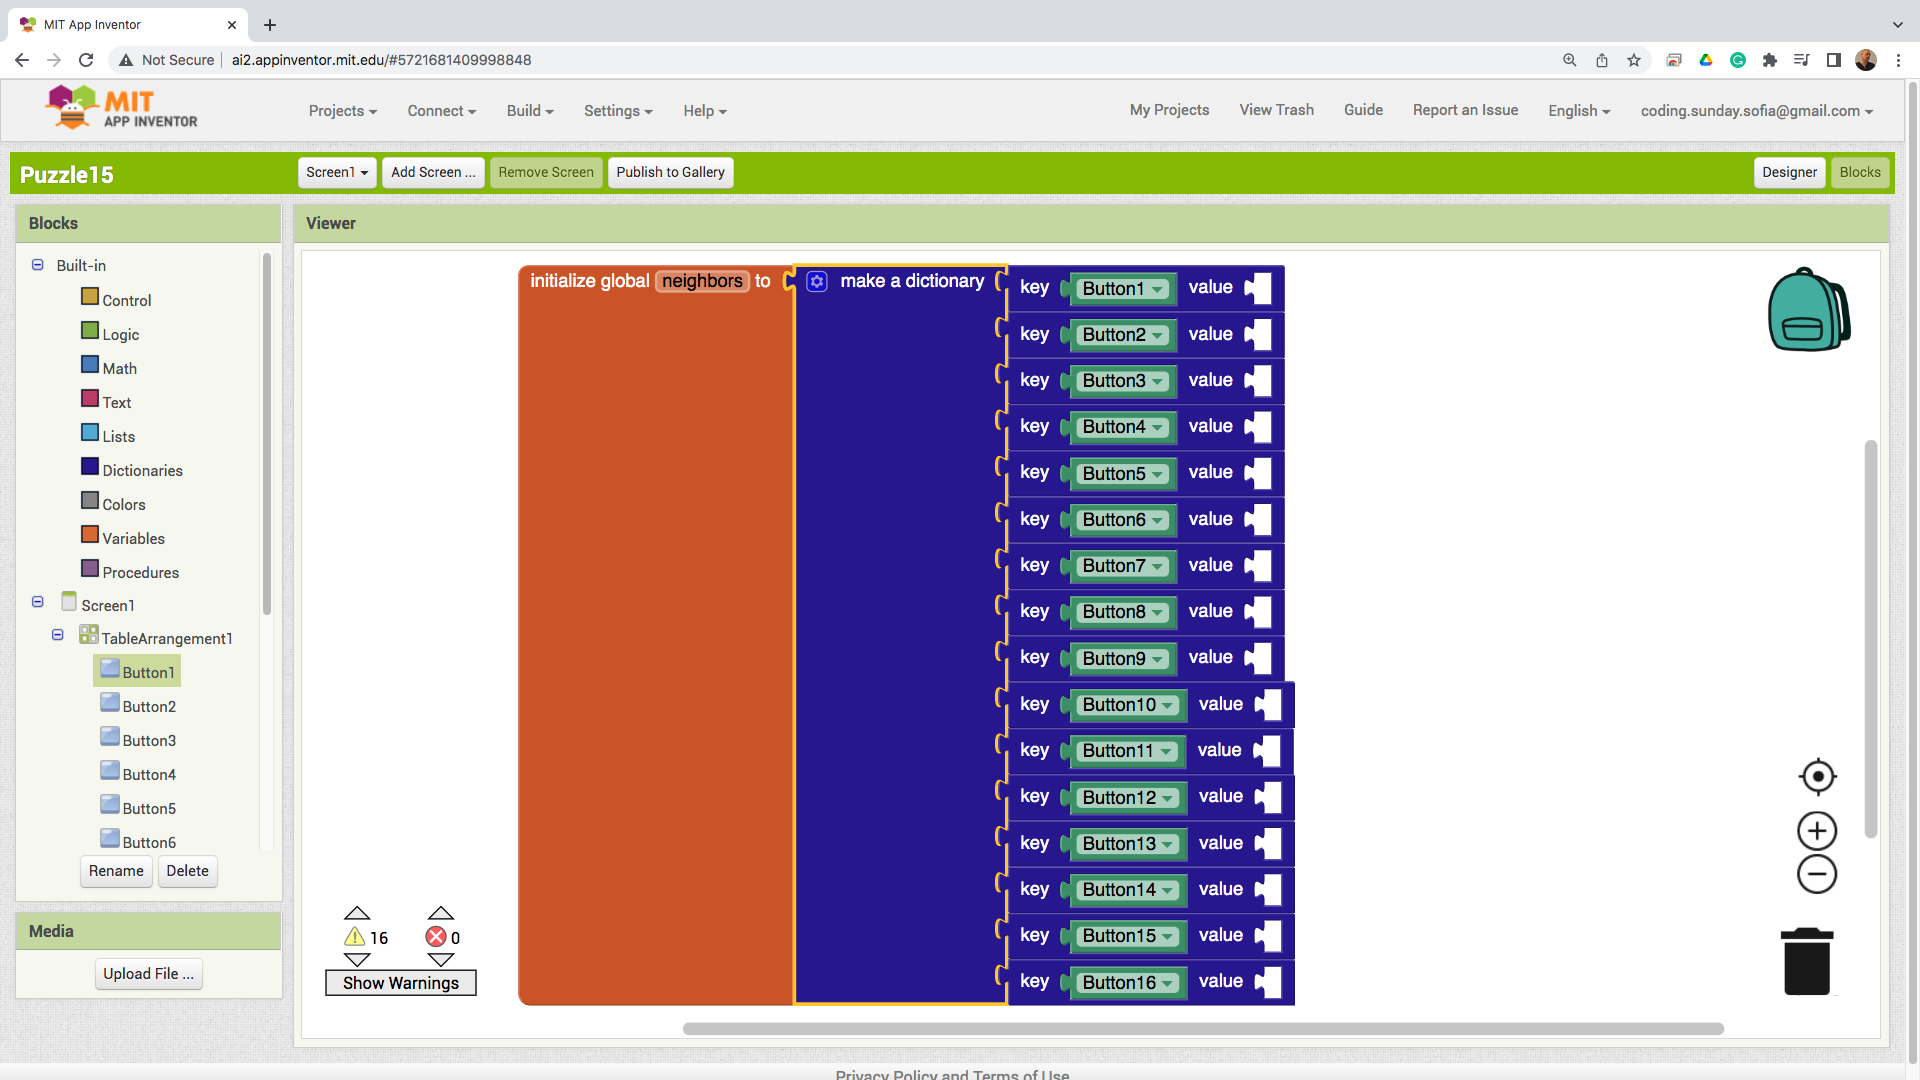
\includegraphics[width=1.0\linewidth,height=0.5\linewidth]{fig060005.png}
   \caption{Buttons as key values}
\label{fig060005}
\end{figure}

\section{Data Structures}

This dictionary of matches is made available as a global variable to be used in the various events of the visual interface. Button one for neighbors has button two and button five (Fig. \ref{fig060006}).

\begin{figure}[H]
   \centering
   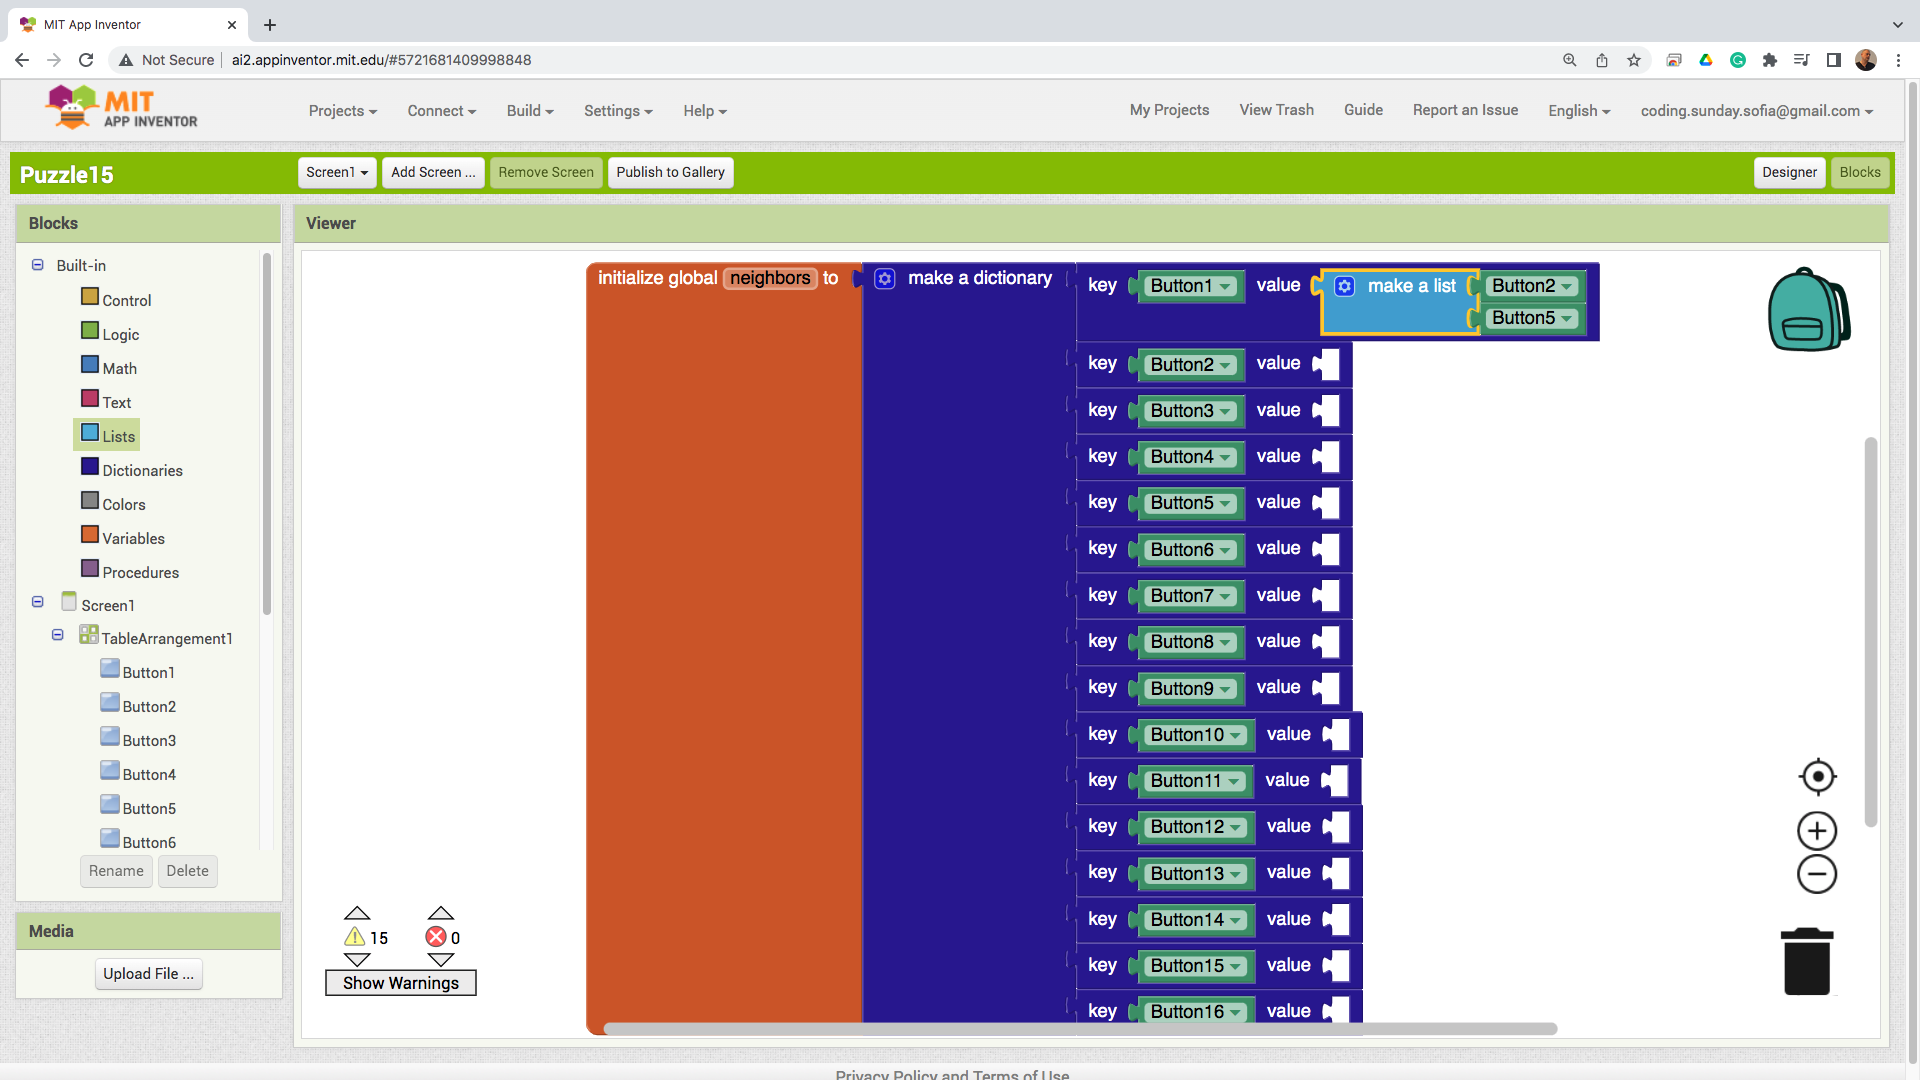
\includegraphics[width=1.0\linewidth,height=0.5\linewidth]{fig060006.png}
   \caption{Buttons as neighbor list}
\label{fig060006}
\end{figure}

Button two has as neighbors buttons one, six and three. Neighbors of button three are two, seven and four. The neighbors of button four are three and eight. Button five's neighbors are one, six, and nine. Neighbors of button six are two, five, seven and ten. Neighbors of button seven are three, six, eight and eleven. Eight's neighbors are four, seven, and twelve. The neighbors of button nine are five, ten and thirteen. Ten's neighbors are six, nine, eleven, and fourteen. The neighbors of button eleven are seven, ten, twelve and fifteen. Button twelve's neighbors are eight, eleven, and sixteen. The neighbors of button thirteen are nine and fourteen. Fourteen's neighbors are ten, thirteen, and fifteen. The neighbors of button fifteen are eleven, fourteen and sixteen. Sixteen's neighbors are twelve and fifteen. Adjacency lists are completed in an identical manner (Fig. \ref{fig060007}).

\begin{figure}[H]
   \centering
   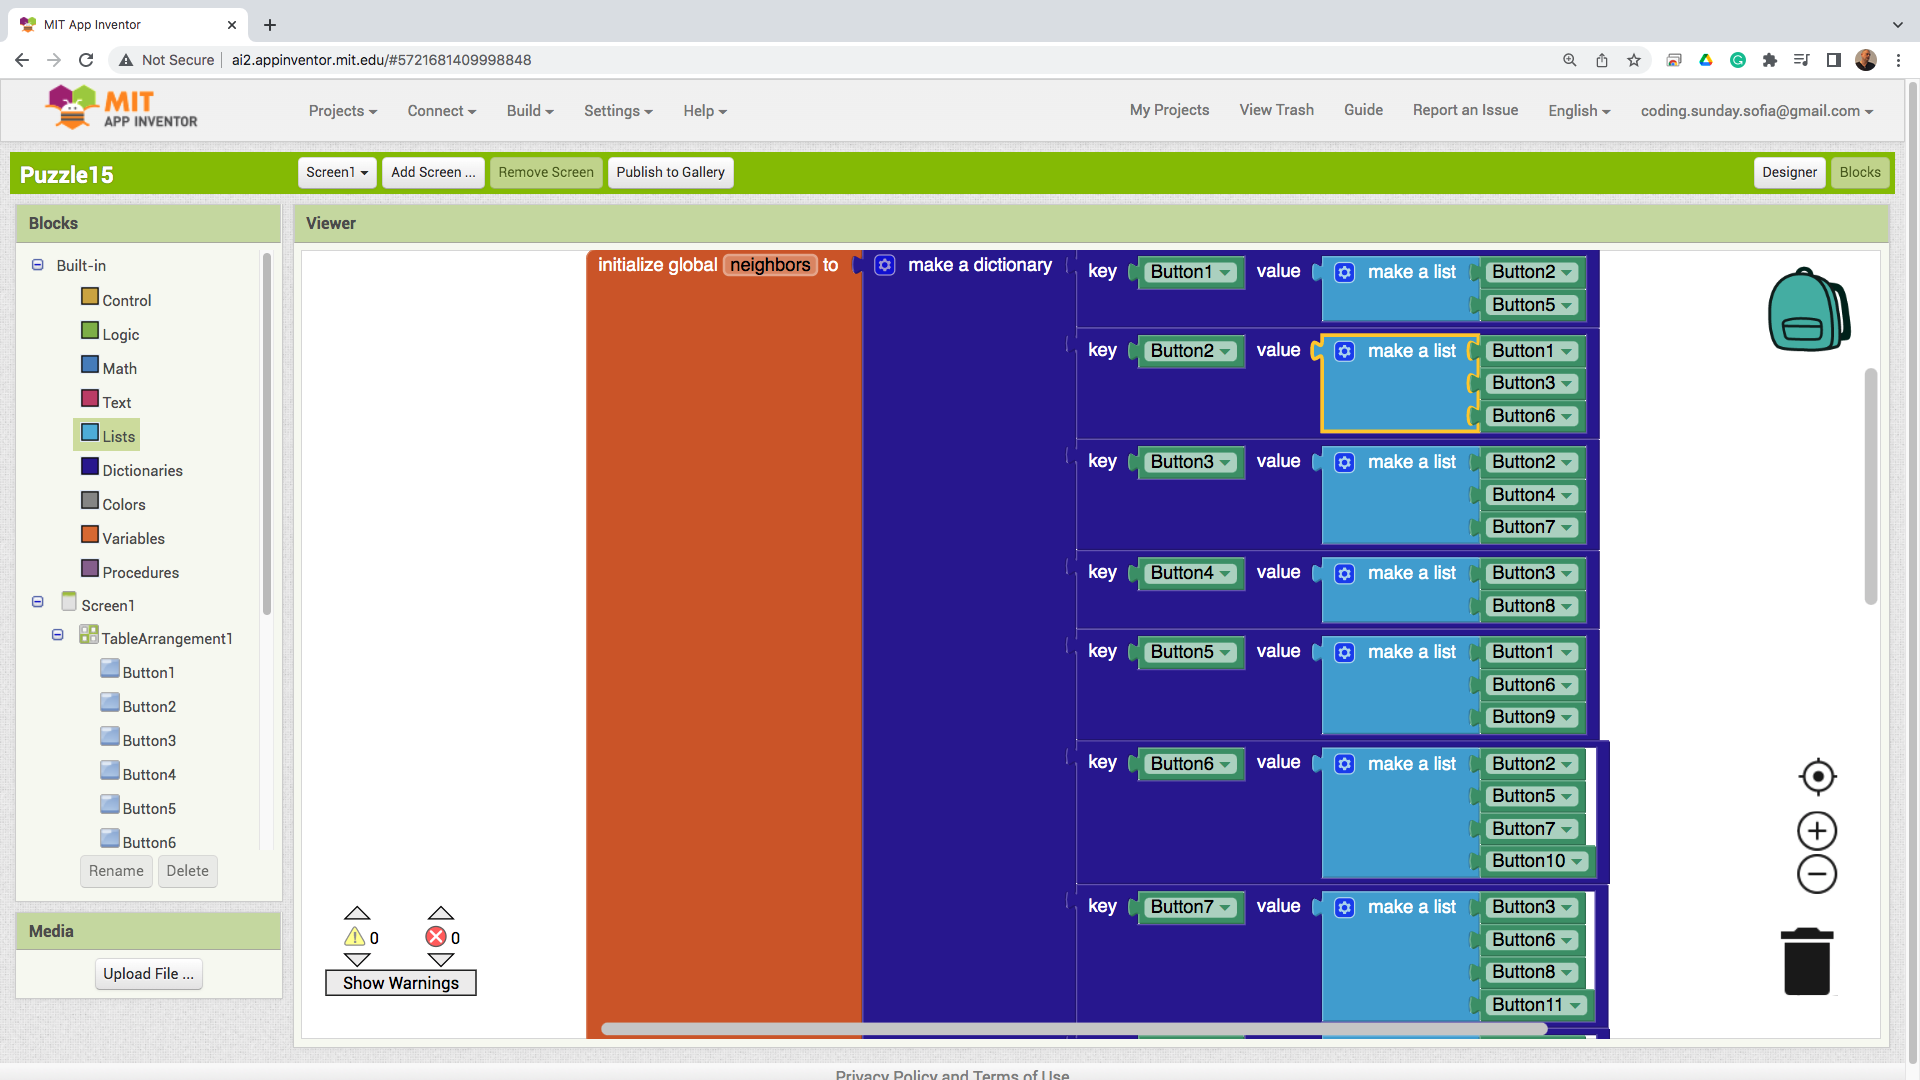
\includegraphics[width=1.0\linewidth,height=0.5\linewidth]{fig060007.png}
   \caption{Identical filling of adjacent buttons}
\label{fig060007}
\end{figure}

Pressing any of the buttons triggers an event that is common to all buttons (Fig. \ref{fig060008}). Since it is not specified which button the user will press, it is checked for the pressed button (comes as an event parameter).

\begin{figure}[H]
   \centering
   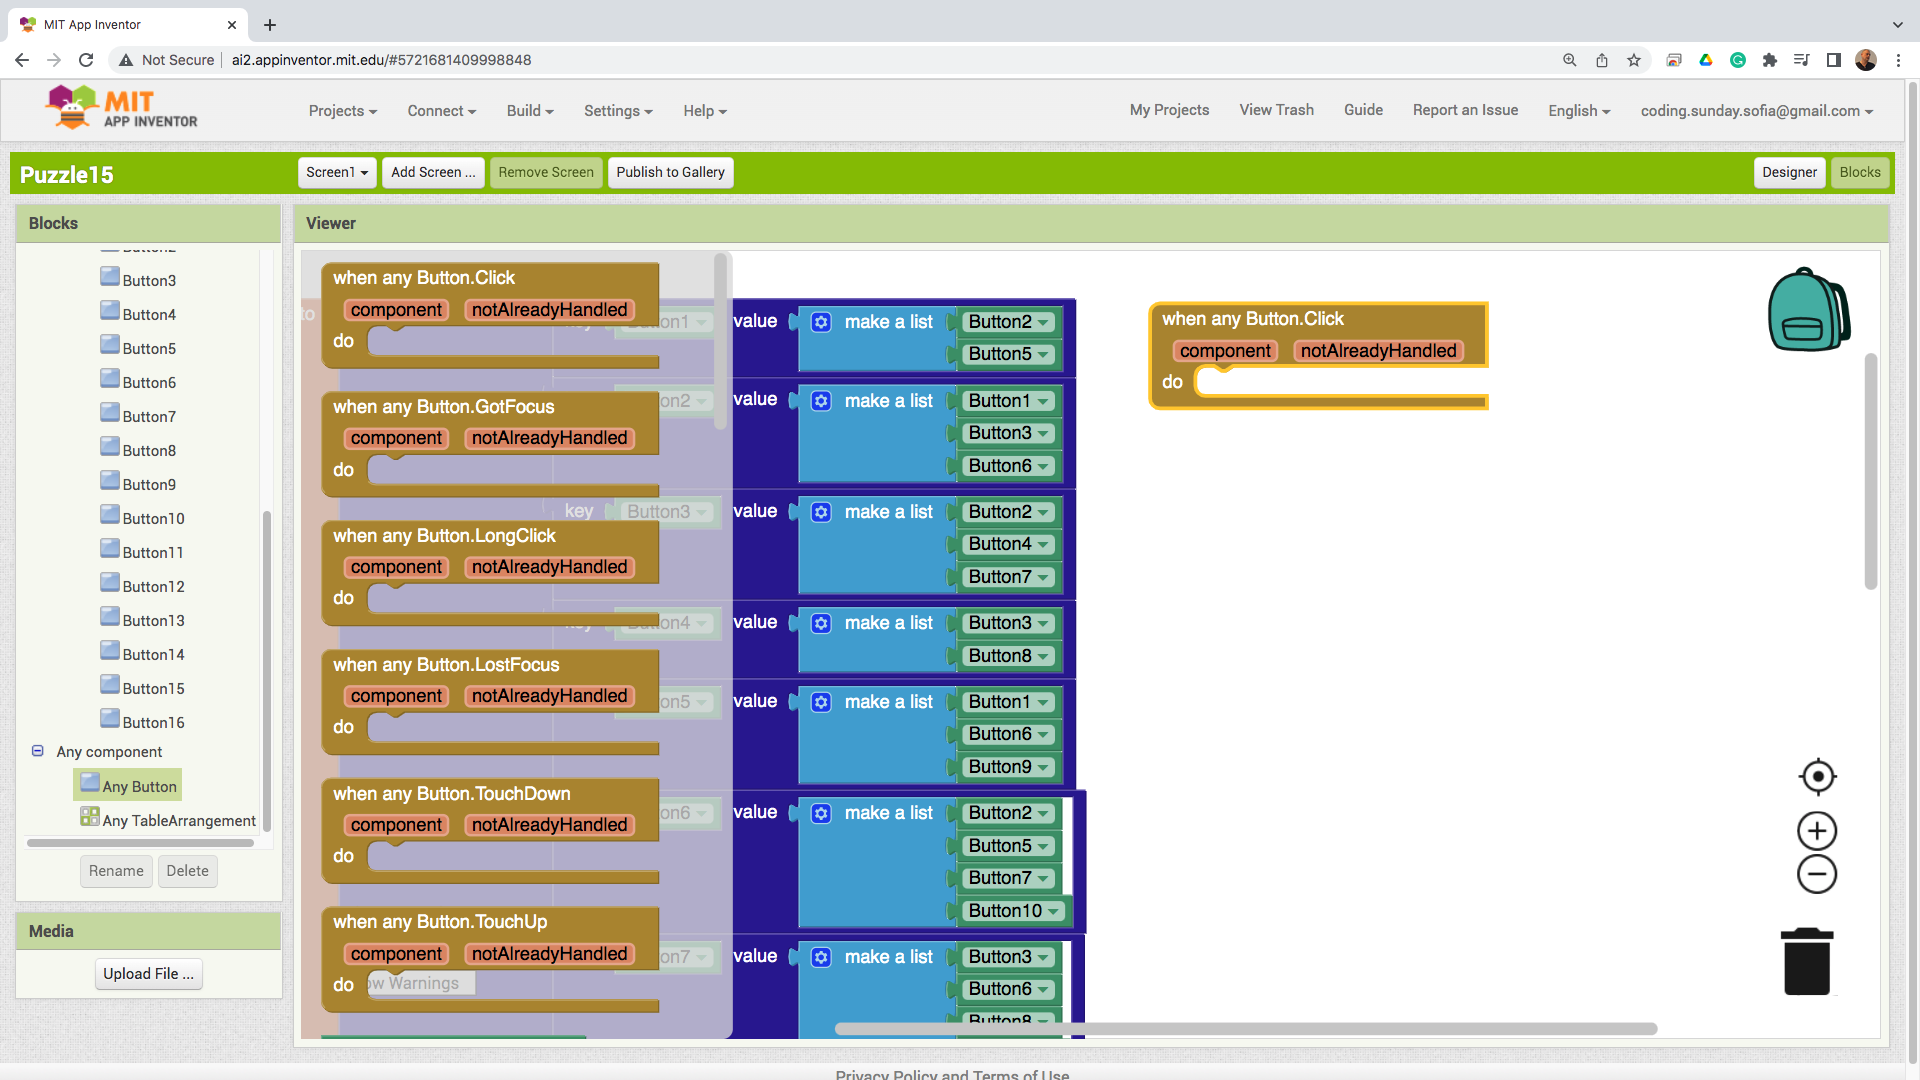
\includegraphics[width=1.0\linewidth,height=0.5\linewidth]{fig060008.png}
   \caption{Button pressed event}
\label{fig060008}
\end{figure}

\section{Game State Handling Algorithms}

The check whether the different cell is a neighbor and the possible exchange with the empty cell is entrusted to an additional procedure (Fig. \ref{fig060009}). The procedure receives as an input parameter the component that caused the event.

\begin{figure}[H]
   \centering
   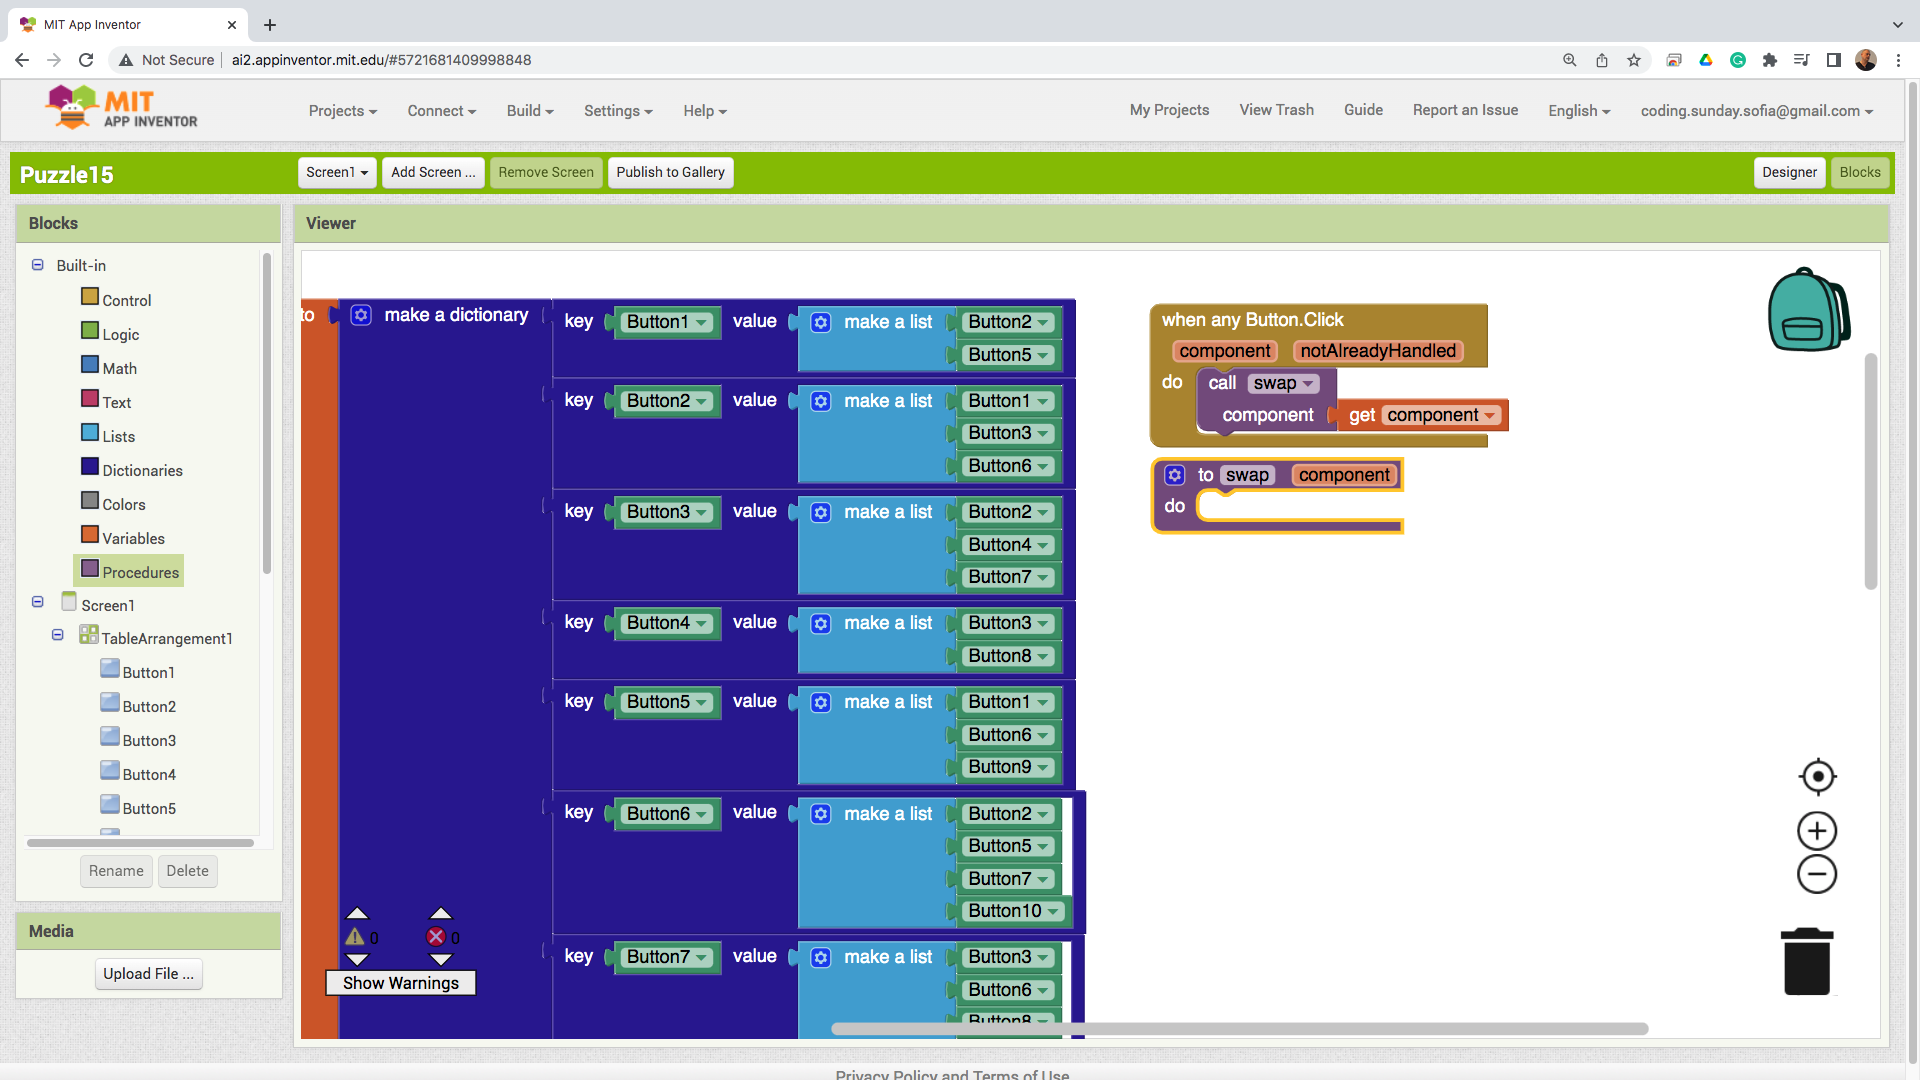
\includegraphics[width=1.0\linewidth,height=0.5\linewidth]{fig060009.png}
   \caption{Exchange Procedure}
\label{fig060009}
\end{figure}

To determine if the empty cell is adjacent to the pressed button, the entire list that is in the dictionary of the key position specified by the component that raised the event is checked. This check is possible with a loop for traversing the elements in a list structure (Fig. \ref{fig060010}). The key value should always return a list of adjacent buttons, but if the key is not found, an empty list is returned to be safe.

\begin{figure}[H]
   \centering
   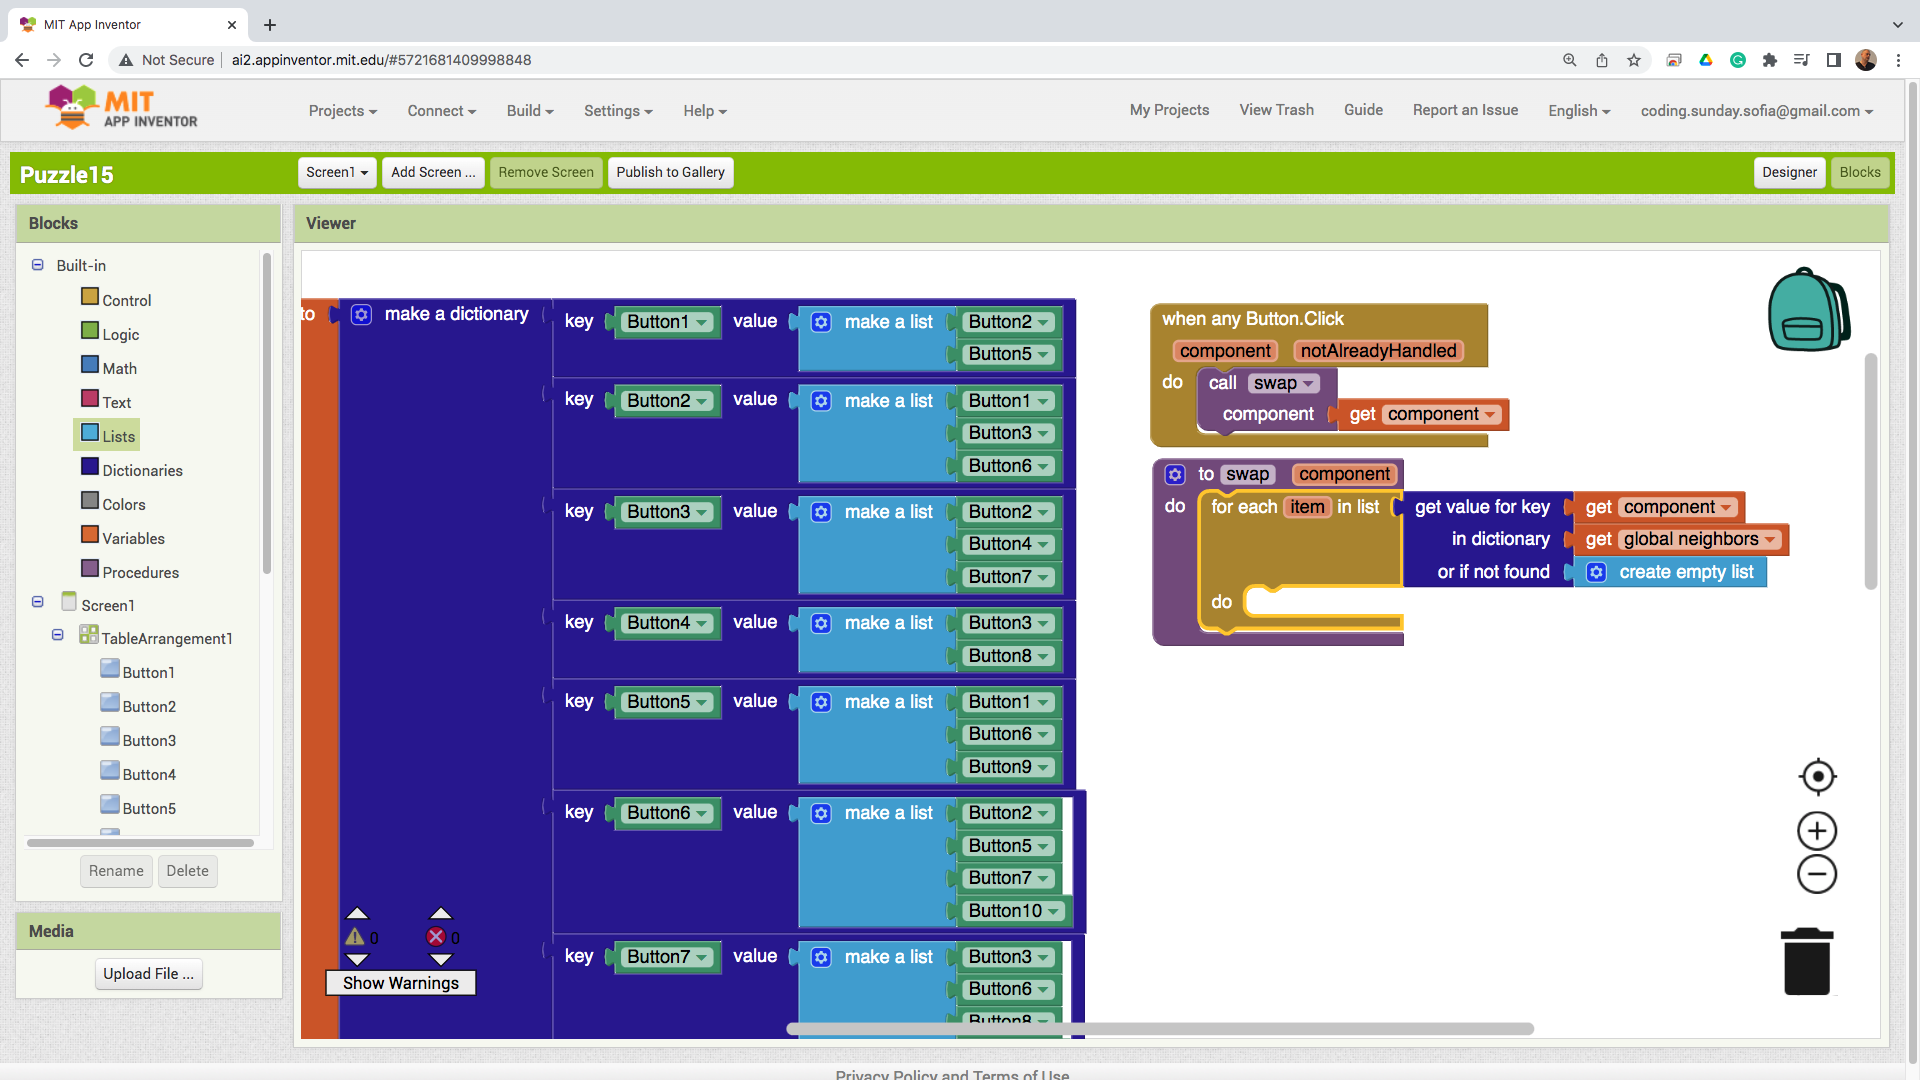
\includegraphics[width=1.0\linewidth,height=0.5\linewidth]{fig060010.png}
   \caption{Neighbor Traversal Cycle}
\label{fig060010}
\end{figure}

Replace with only if the empty cell is found in the list. Doing the swap also stops the cycle of looking for the empty cell. The condition for an adjacent button to indicate the washed cell is that its label should be two spaces (Fig. \ref{fig060011}).

\begin{figure}[H]
   \centering
   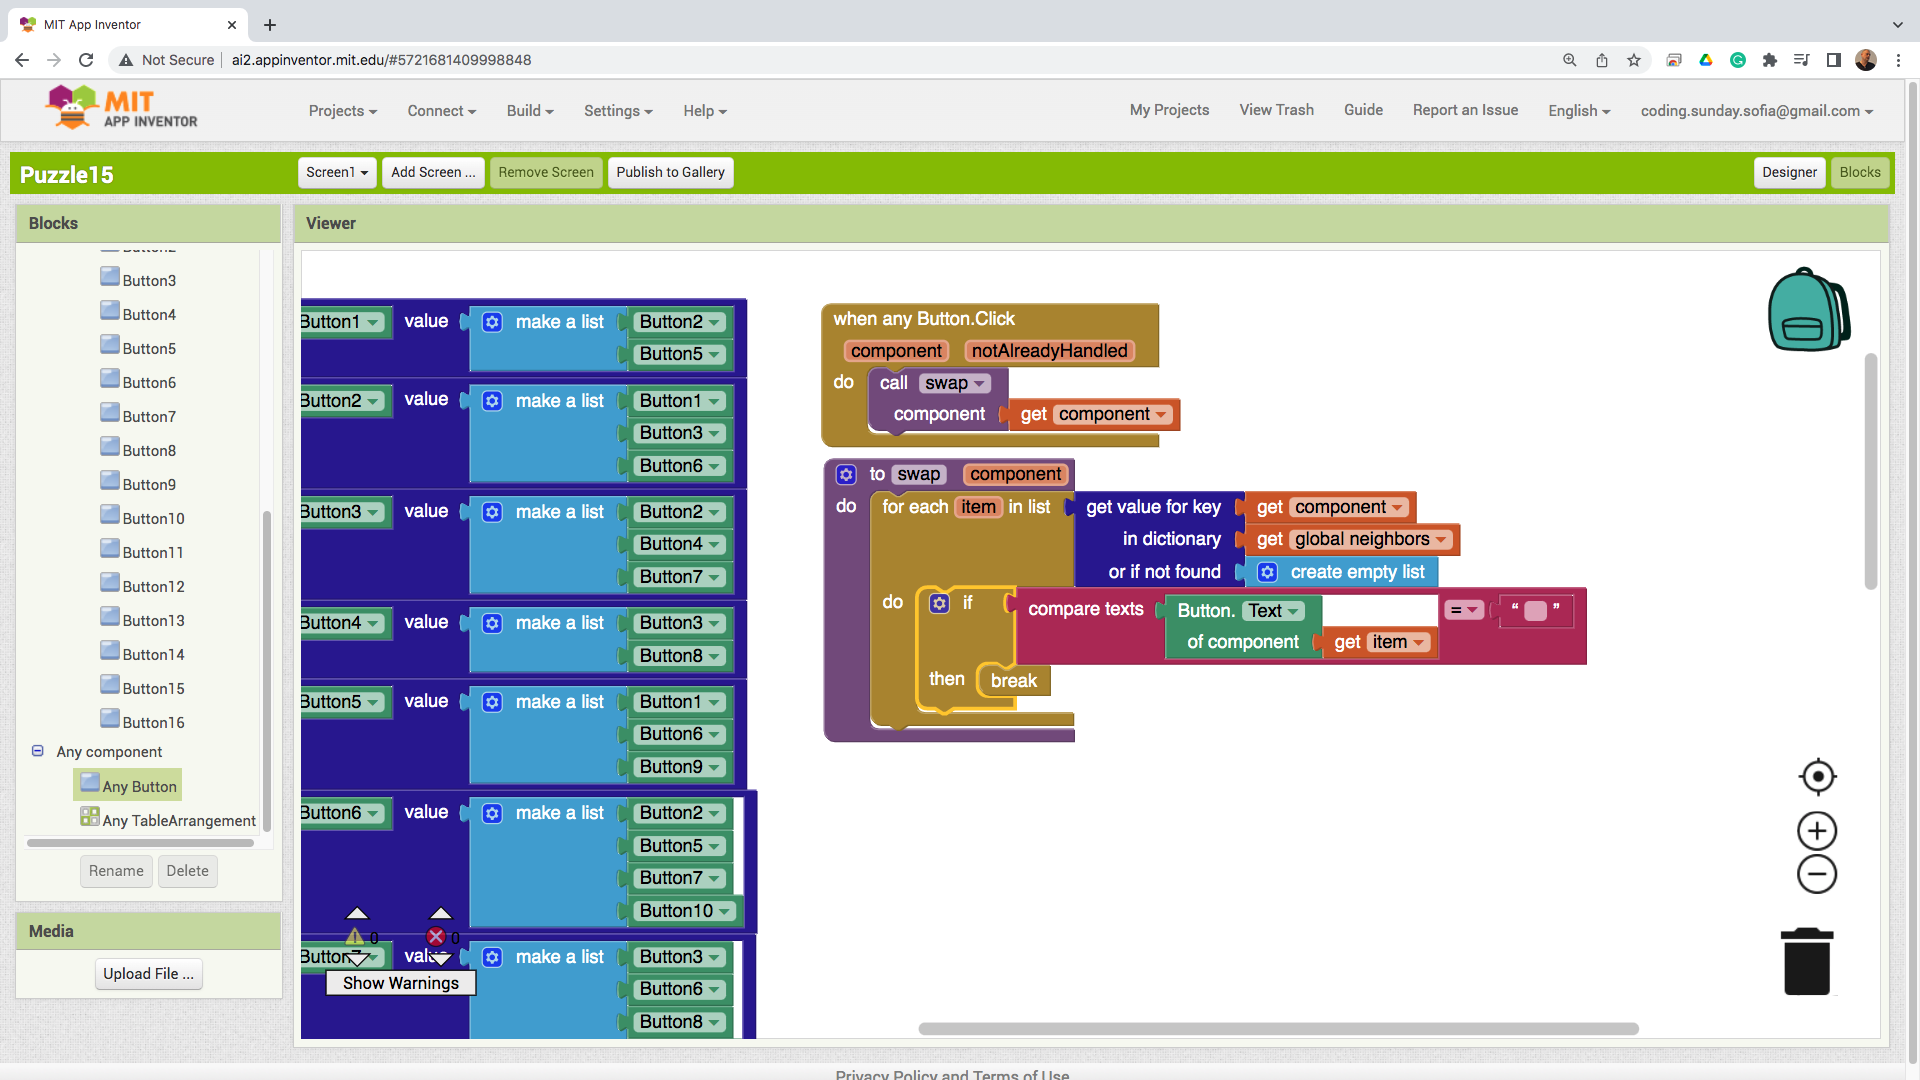
\includegraphics[width=1.0\linewidth,height=0.5\linewidth]{fig060011.png}
   \caption{Checking for the empty cell}
\label{fig060011}
\end{figure}

To facilitate the exchange, four local, helper variables are set. Two variables for the texts of the two buttons and two variables for the colors of the texts (Fig. \ref{fig060012}).

\begin{figure}[H]
   \centering
   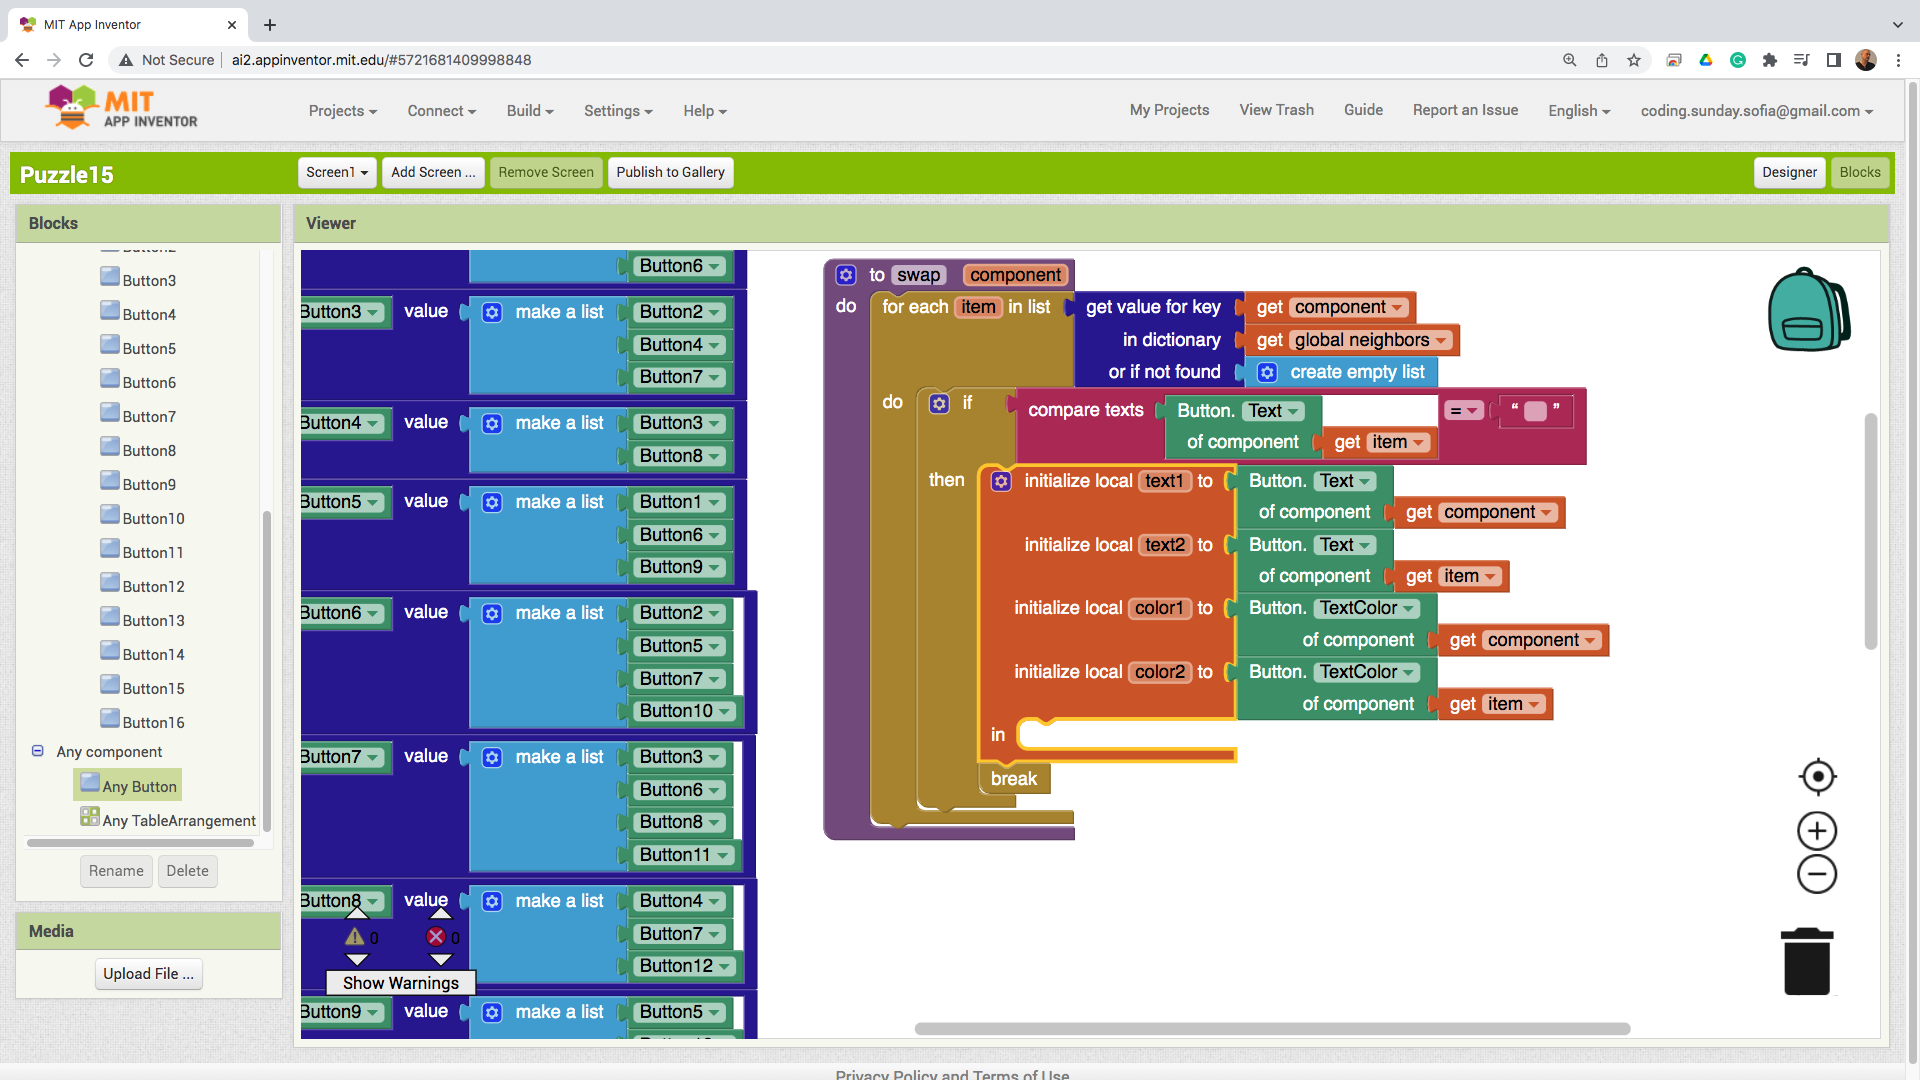
\includegraphics[width=1.0\linewidth,height=0.5\linewidth]{fig060012.png}
   \caption{Local Helper Variables}
\label{fig060012}
\end{figure}

The exchange is done by writing the auxiliary variables as new values for the two buttons (Fig. \ref{fig060013}).

\begin{figure}[H]
   \centering
   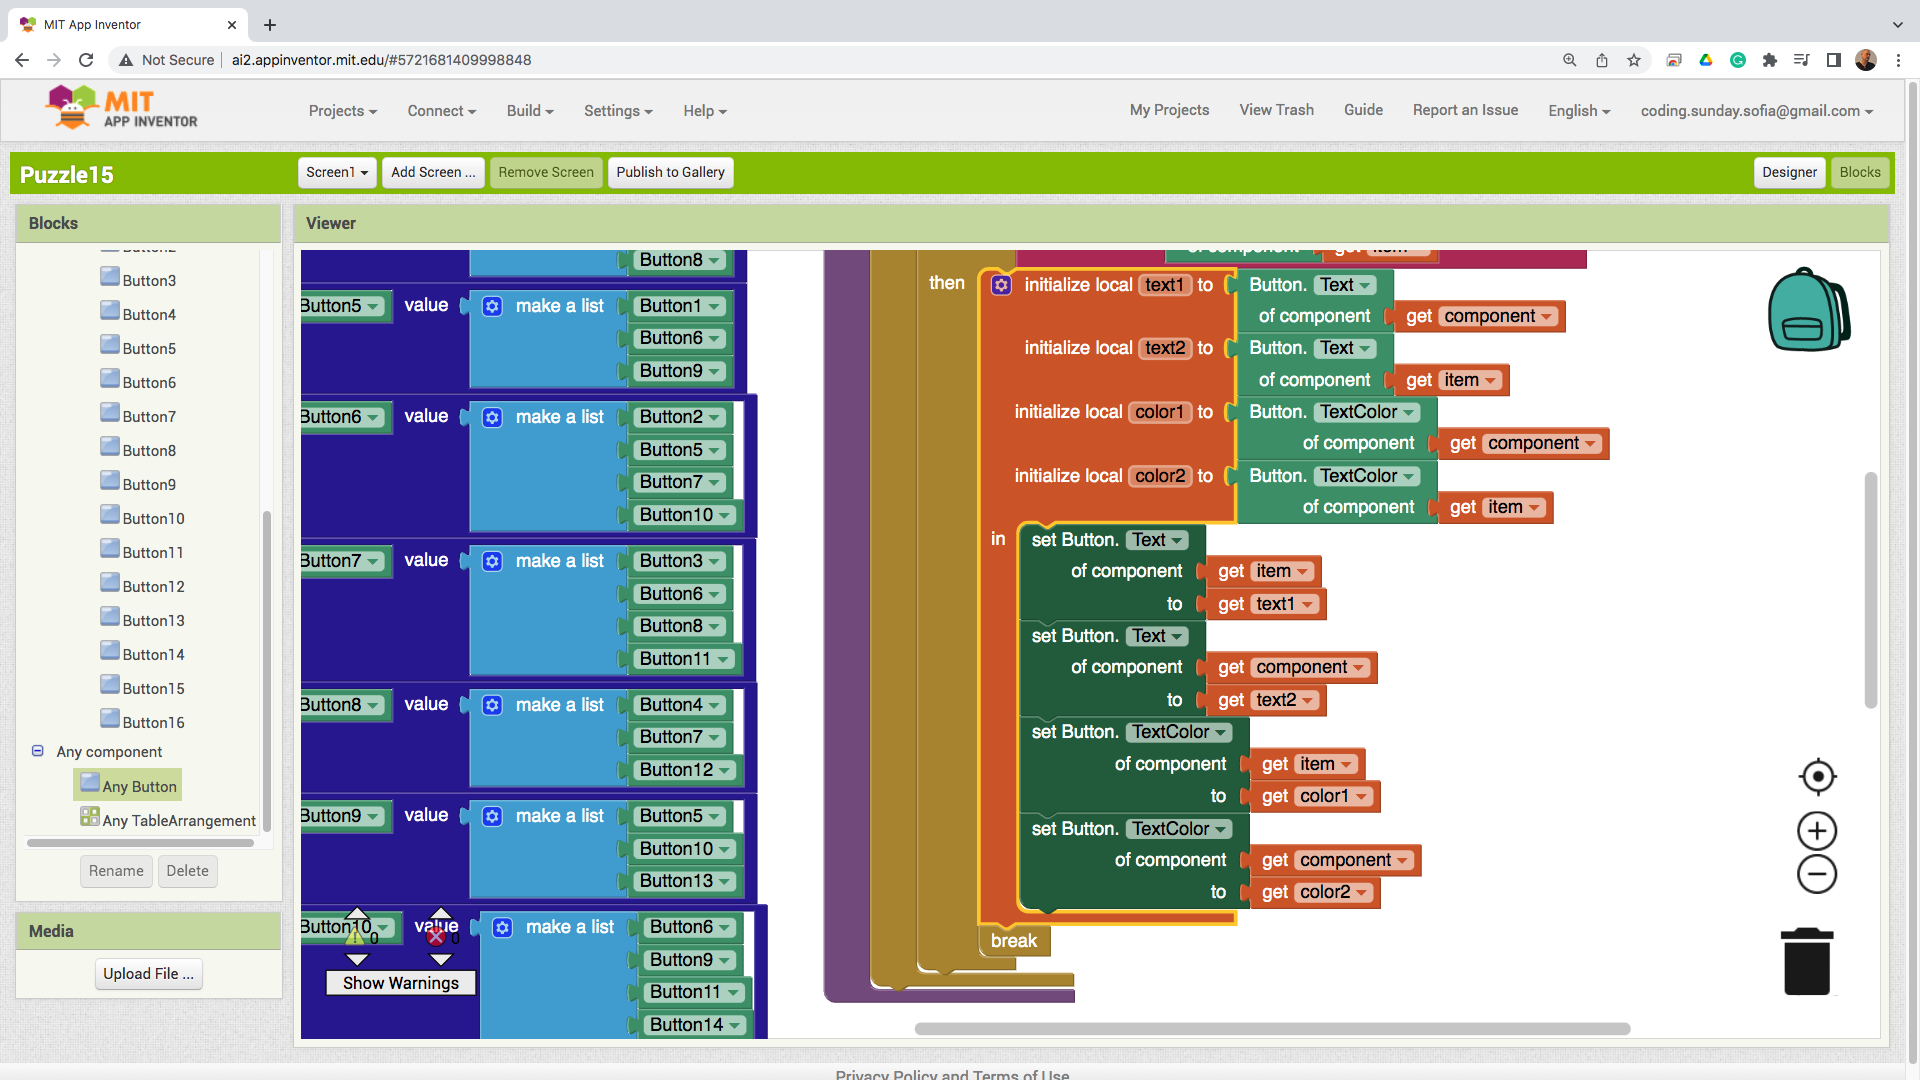
\includegraphics[width=1.0\linewidth,height=0.5\linewidth]{fig060013.png}
   \caption{Swap Values}
\label{fig060013}
\end{figure}

At this stage, the game has absolutely all the functionality that the mechanical toy has (Fig. \ref{fig060014}).

\begin{figure}[H]
   \centering
   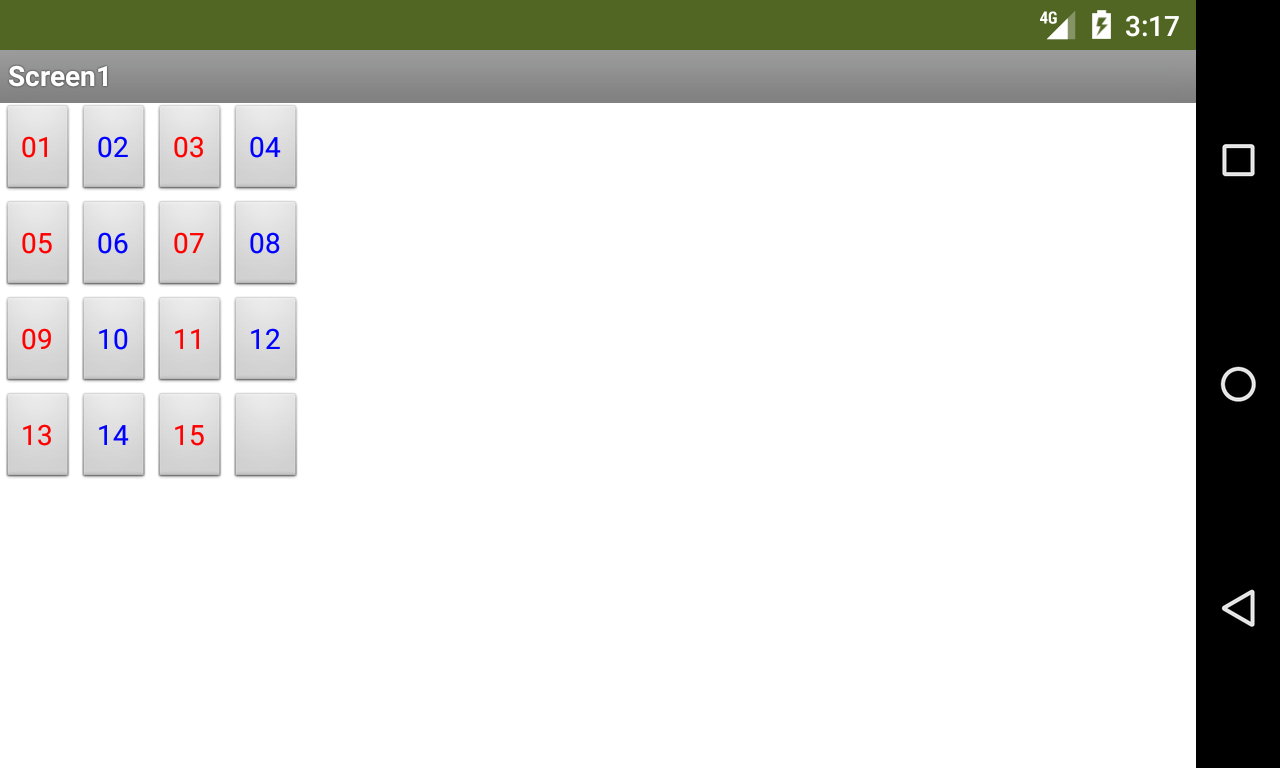
\includegraphics[width=1.0\linewidth,height=0.5\linewidth]{fig060014.png}
   \caption{Finished Game View}
\label{fig060014}
\end{figure}

Although everything you need is available, the use of a computer allows one more useful feature to be added, namely automatic puzzle shuffling. The operating system allows a long press event to be intercepted (Fig. \ref{fig060015}).

\begin{figure}[H]
   \centering
   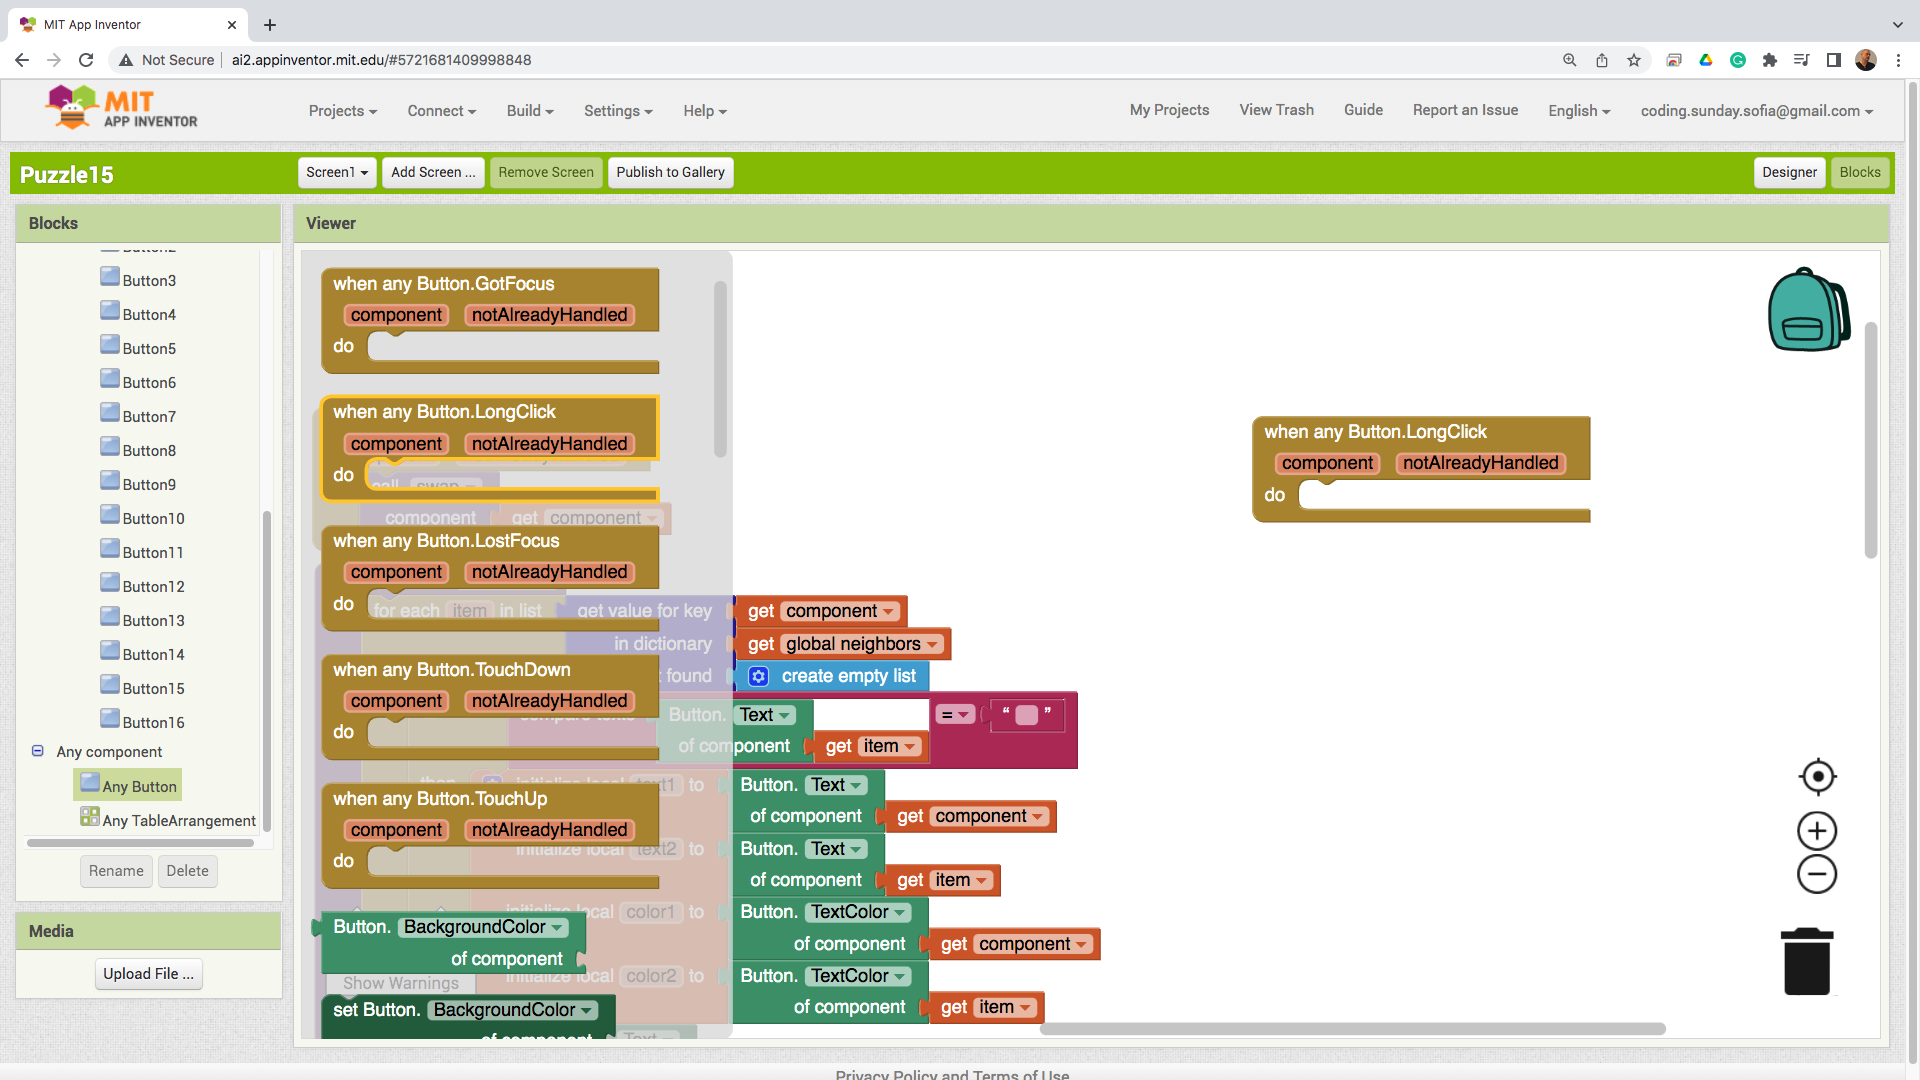
\includegraphics[width=1.0\linewidth,height=0.5\linewidth]{fig060015.png}
   \caption{Button Long Press Event}
\label{fig060015}
\end{figure}

The empty cell button is not loaded with many actions and therefore can be used just like a shuffle button as long as it is pressed for a long time (Fig. \ref{fig060016}).

\begin{figure}[H]
   \centering
   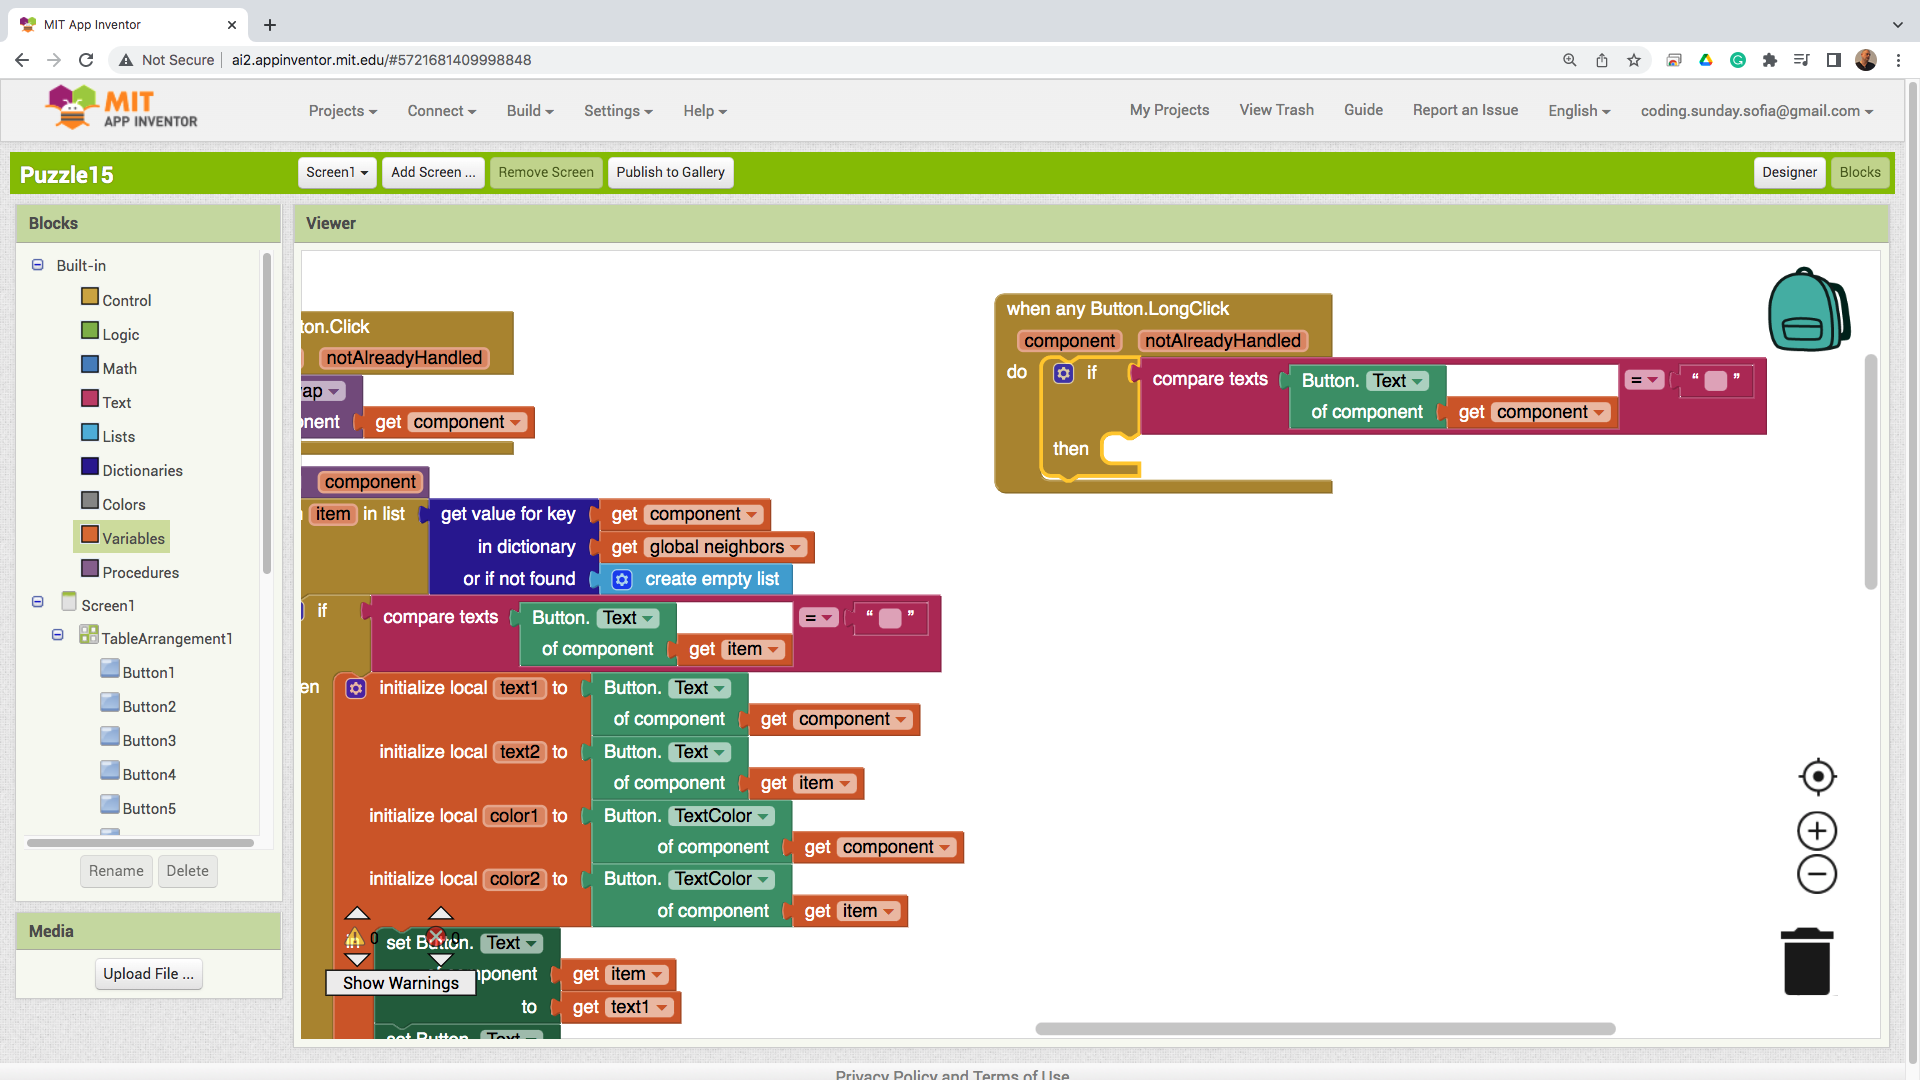
\includegraphics[width=1.0\linewidth,height=0.5\linewidth]{fig060016.png}
   \caption{Enable Shuffle}
\label{fig060016}
\end{figure}

Since the empty cell will move during shuffling, it is a good idea to store its position in a local, helper variable (Fig. \ref{fig060017}).

\begin{figure}[H]
   \centering
   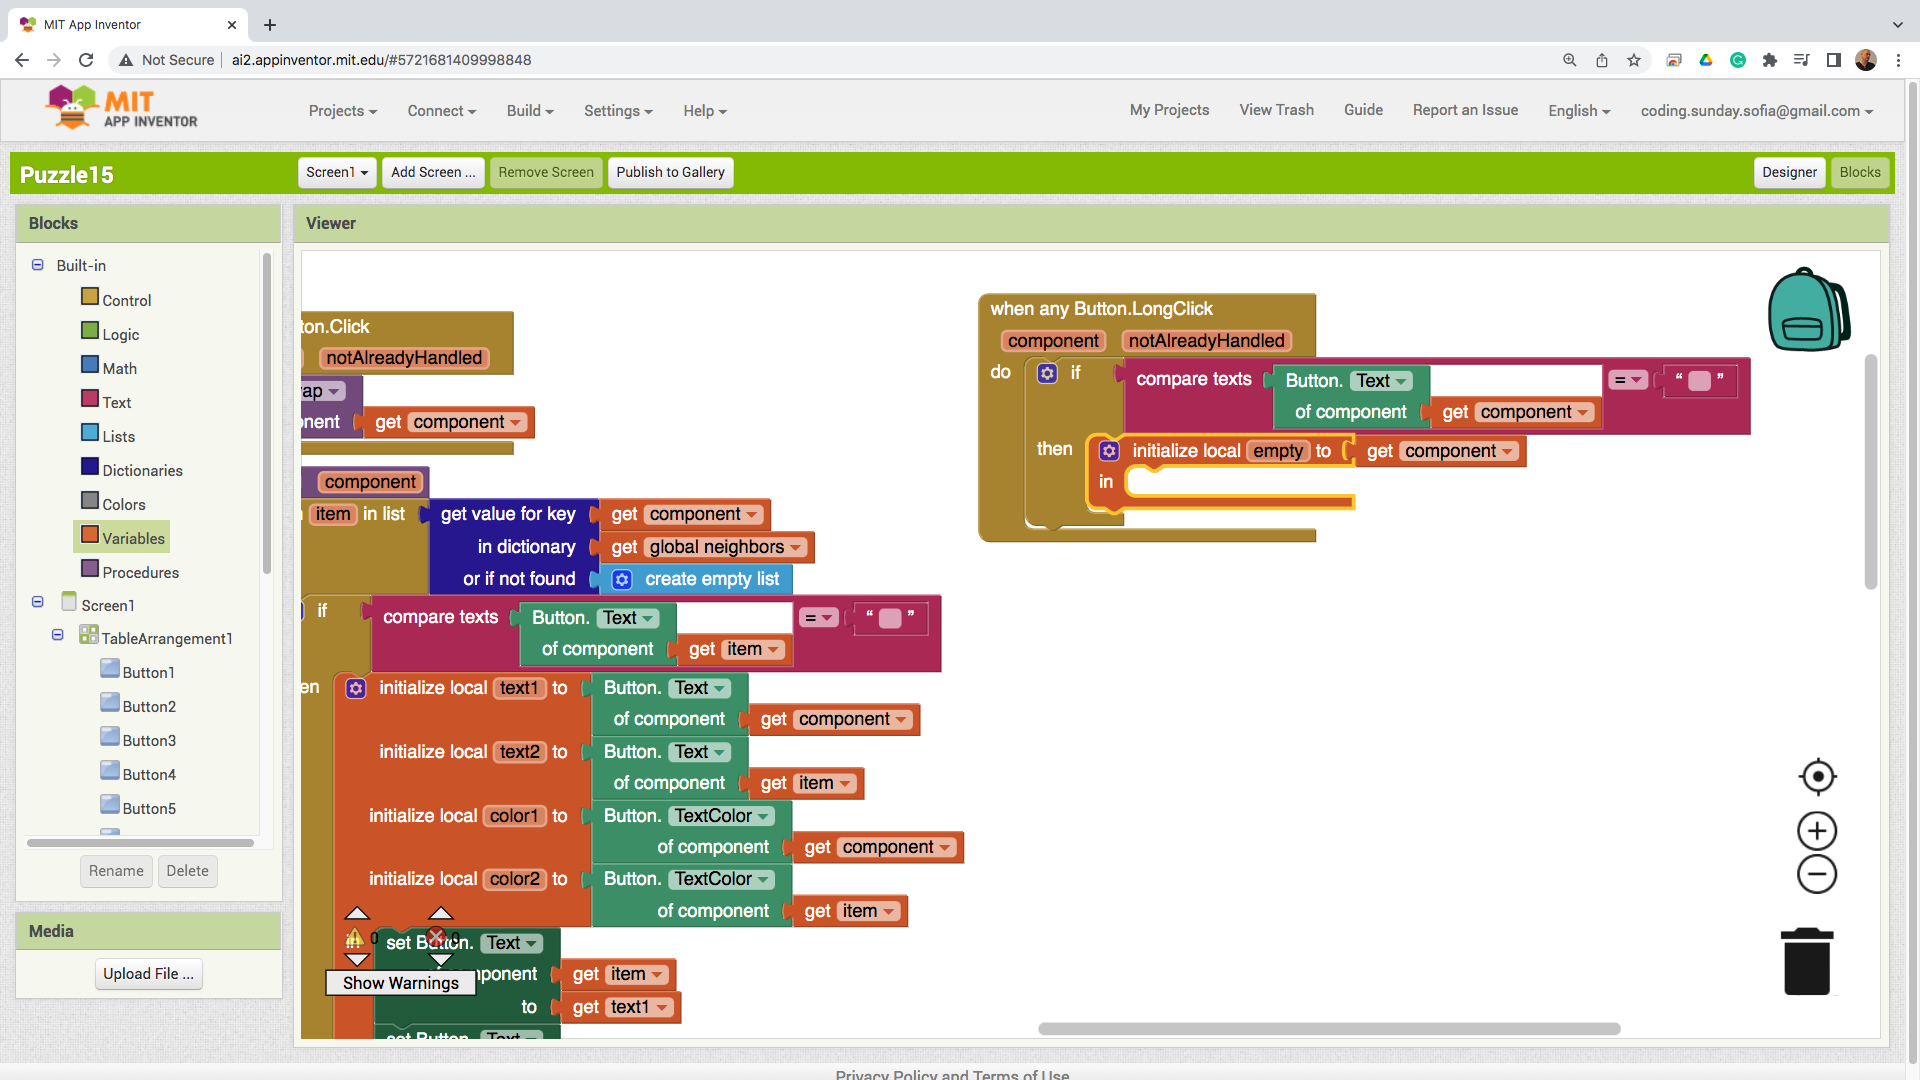
\includegraphics[width=1.0\linewidth,height=0.5\linewidth]{fig060017.png}
   \caption{Helper variable for empty cell position}
\label{fig060017}
\end{figure}

The game board consists of 16 positions. In order for each position to participate, statistically, 10 times in the shuffle, randomly chosen shuffles can be made 160 times, which is 16 cells ten times. For the purpose of stirring, a single-step loop is the most suitable design (Fig. \ref{fig060018}).

\begin{figure}[H]
   \centering
   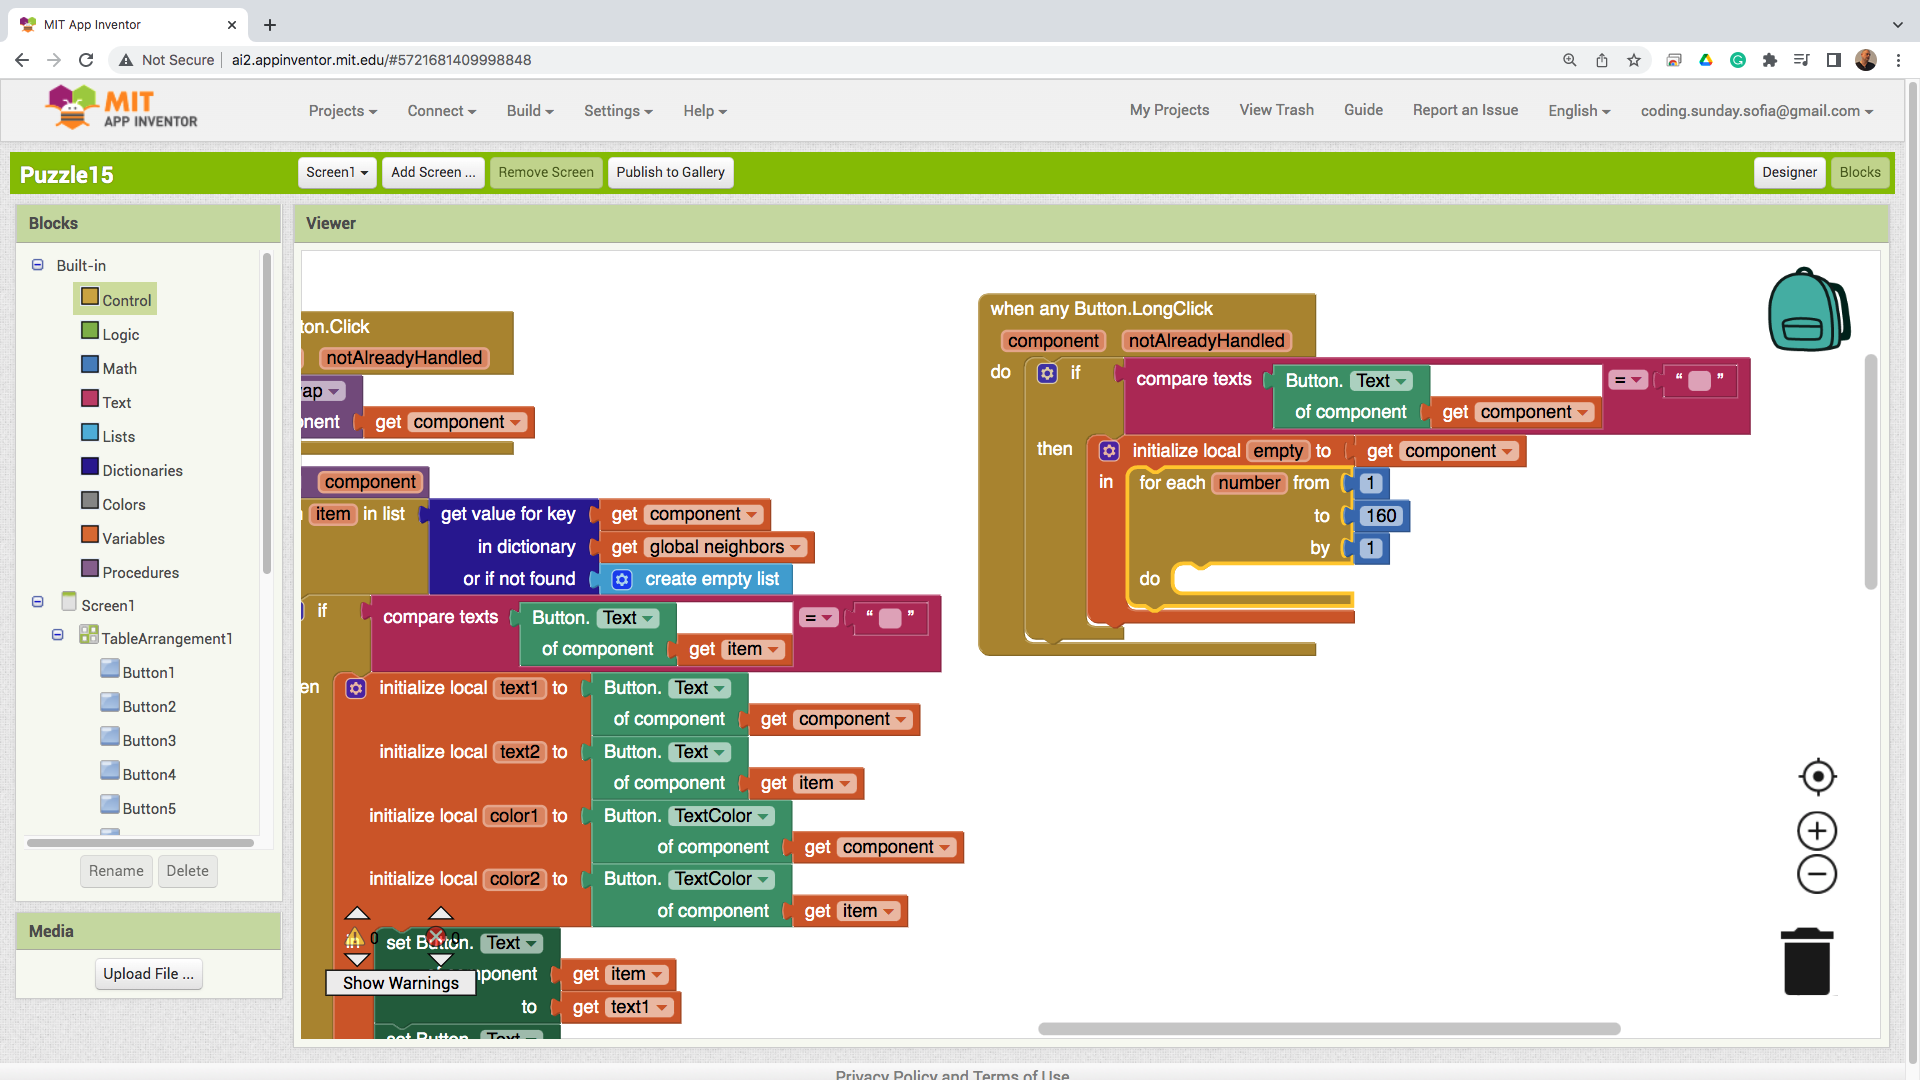
\includegraphics[width=1.0\linewidth,height=0.5\linewidth]{fig060018.png}
   \caption{Shuffle Loop}
\label{fig060018}
\end{figure}

The next empty cell is chosen randomly from the neighbors of the current empty cell (Fig. \ref{fig060019}). The next empty cell is written to a temporary variable until the swap is done.

\begin{figure}[H]
   \centering
   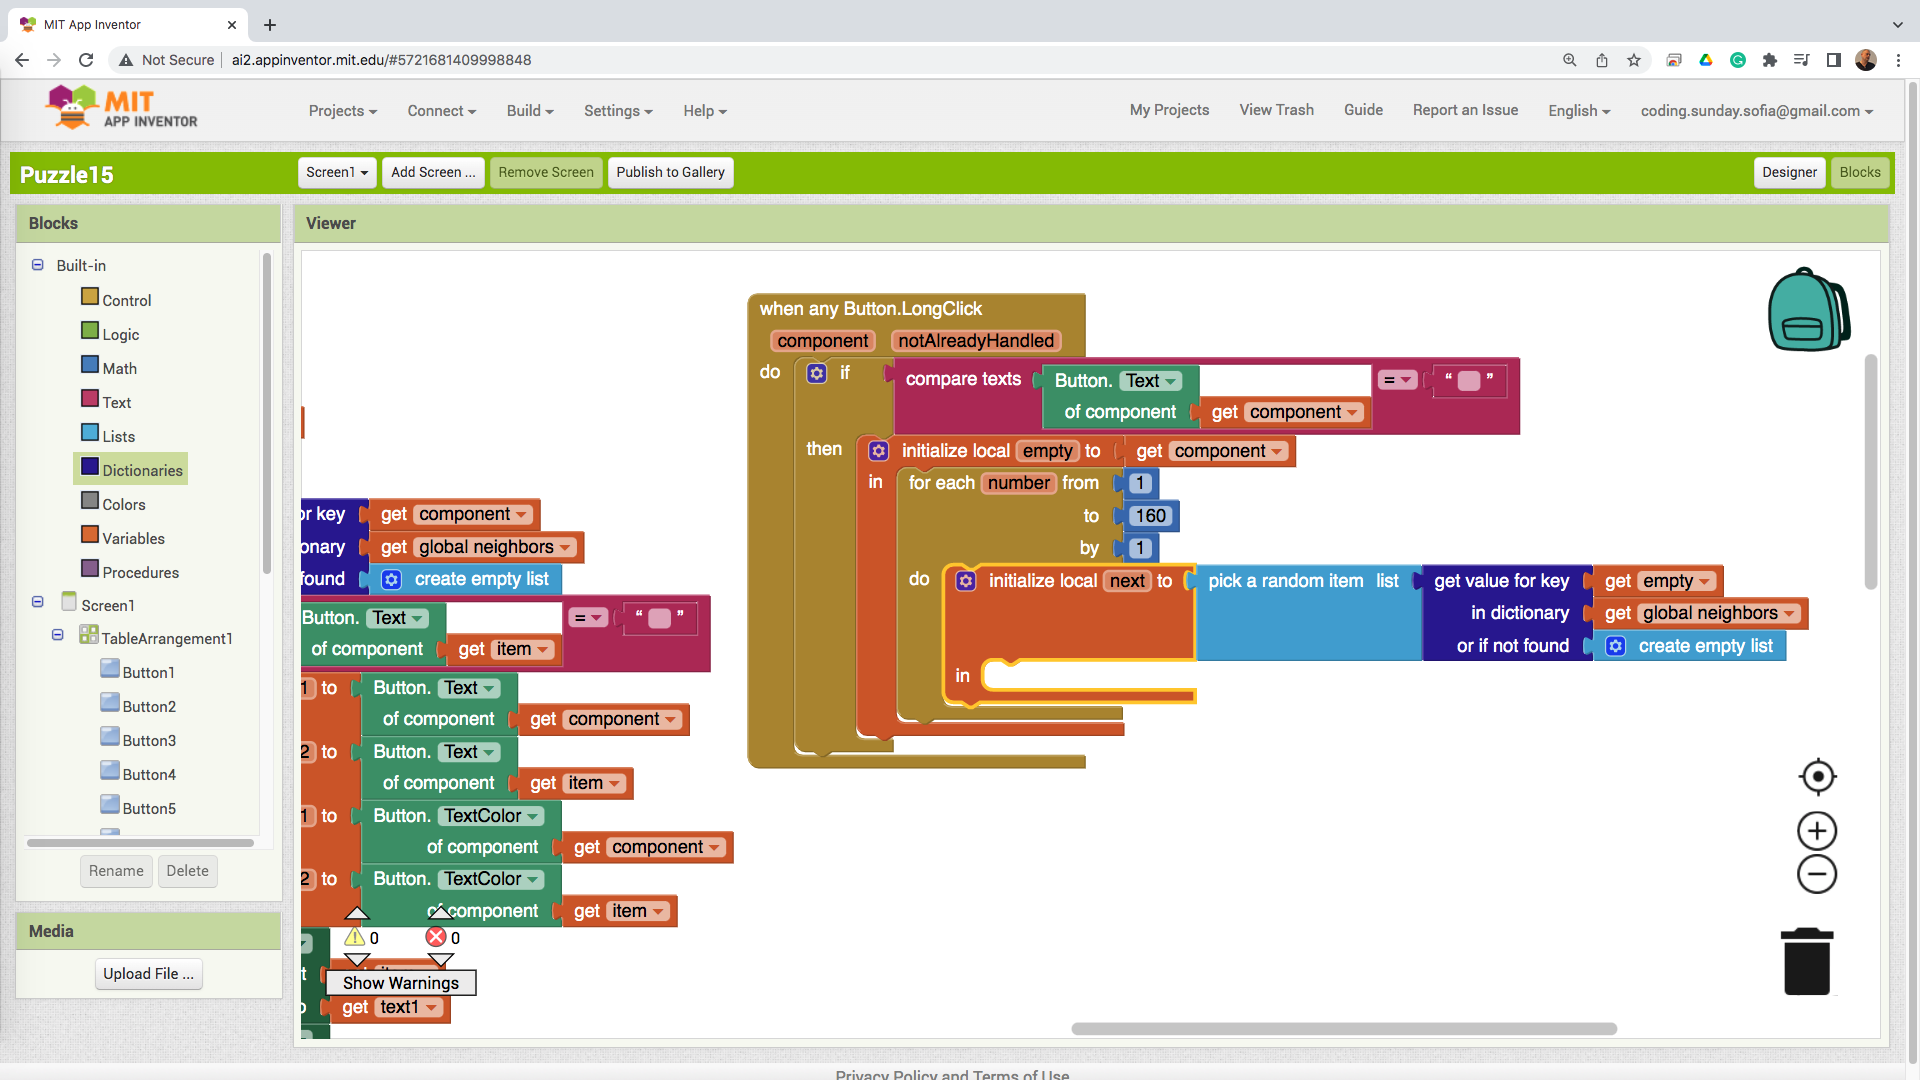
\includegraphics[width=1.0\linewidth,height=0.5\linewidth]{fig060019.png}
   \caption{Choosing a random neighbor of the empty cell}
\label{fig060019}
\end{figure}

The exchange itself is carried out with the auxiliary procedure (Fig. \ref{fig060020}). After the swap, the empty cell for the next spin of the loop is swapped.

\begin{figure}[H]
   \centering
   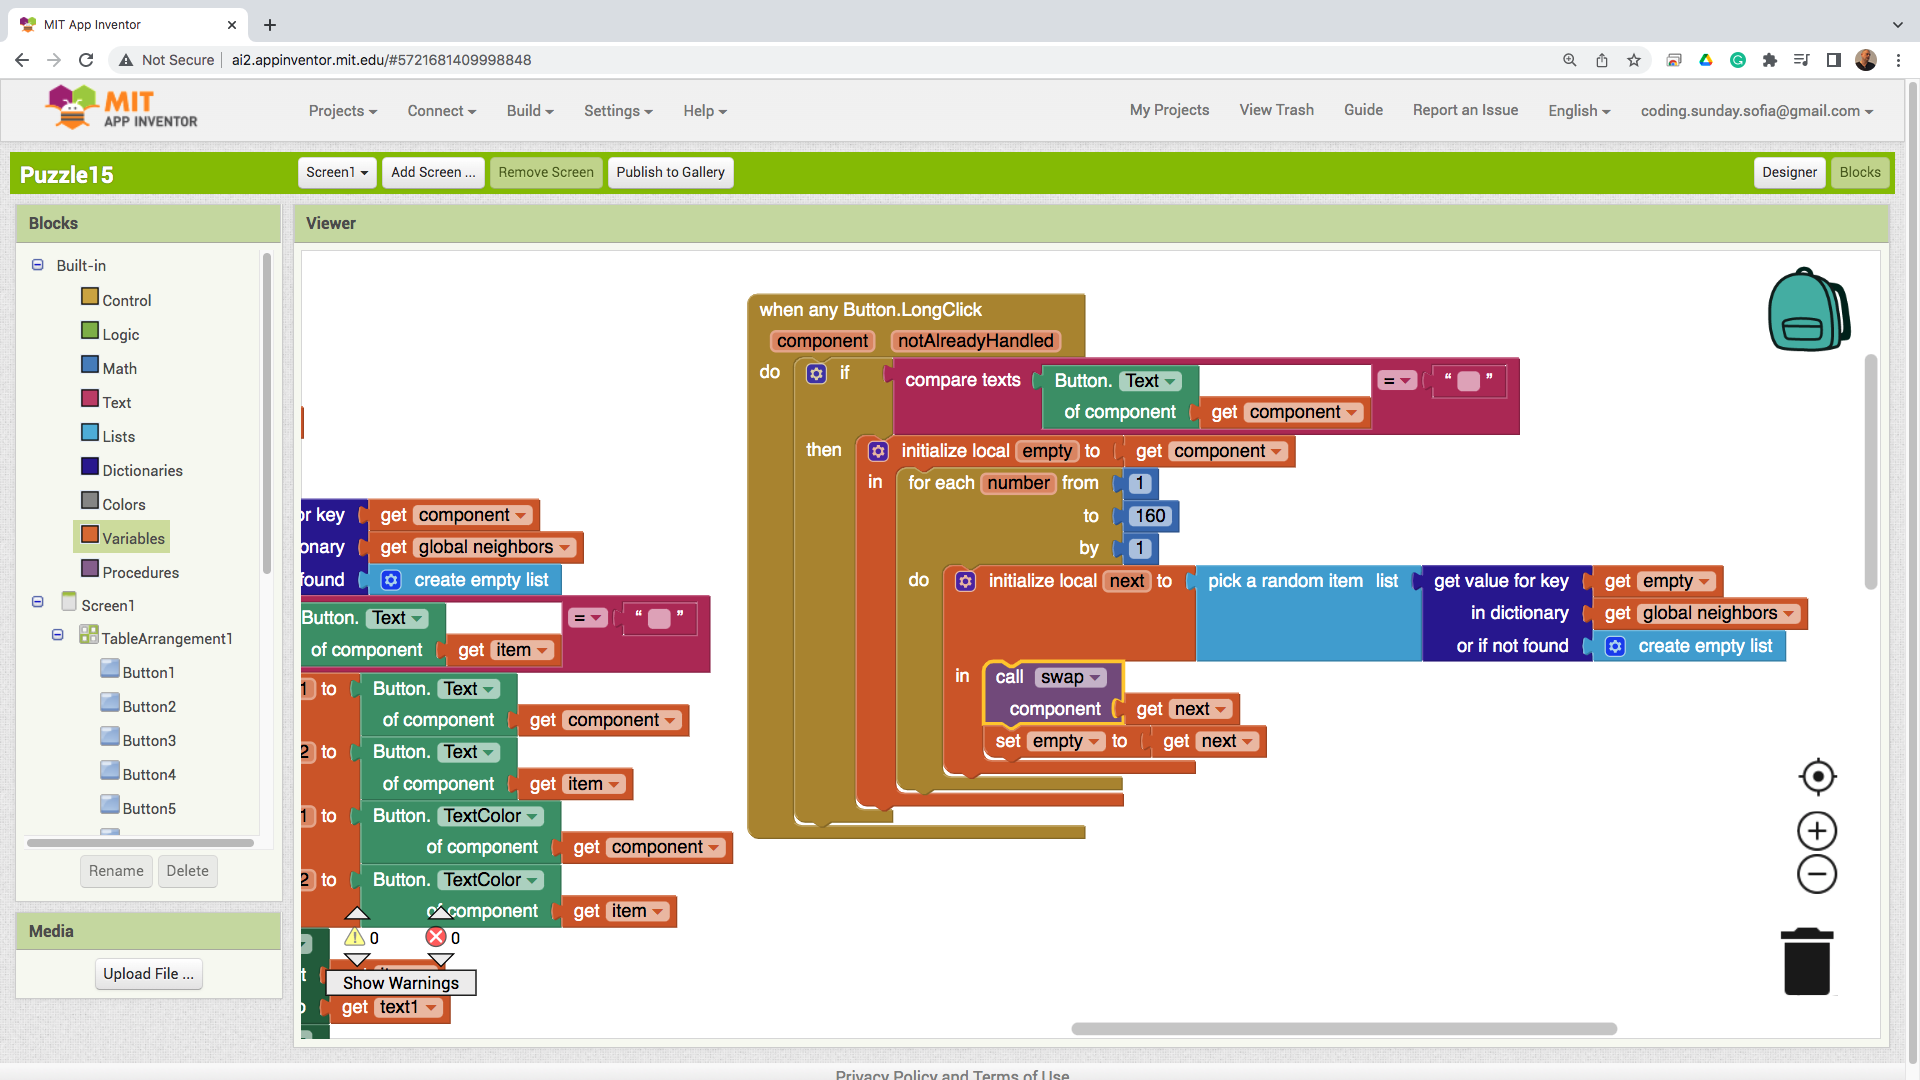
\includegraphics[width=1.0\linewidth,height=0.5\linewidth]{fig060020.png}
   \caption{Swap the empty cell}
\label{fig060020}
\end{figure}

\section{Publish the project}

After the game is completed, the project can be published to the general audience using the "Publish to Gallery" button (Fig. \ref{fig060021}).

\begin{figure}[H]
   \centering
   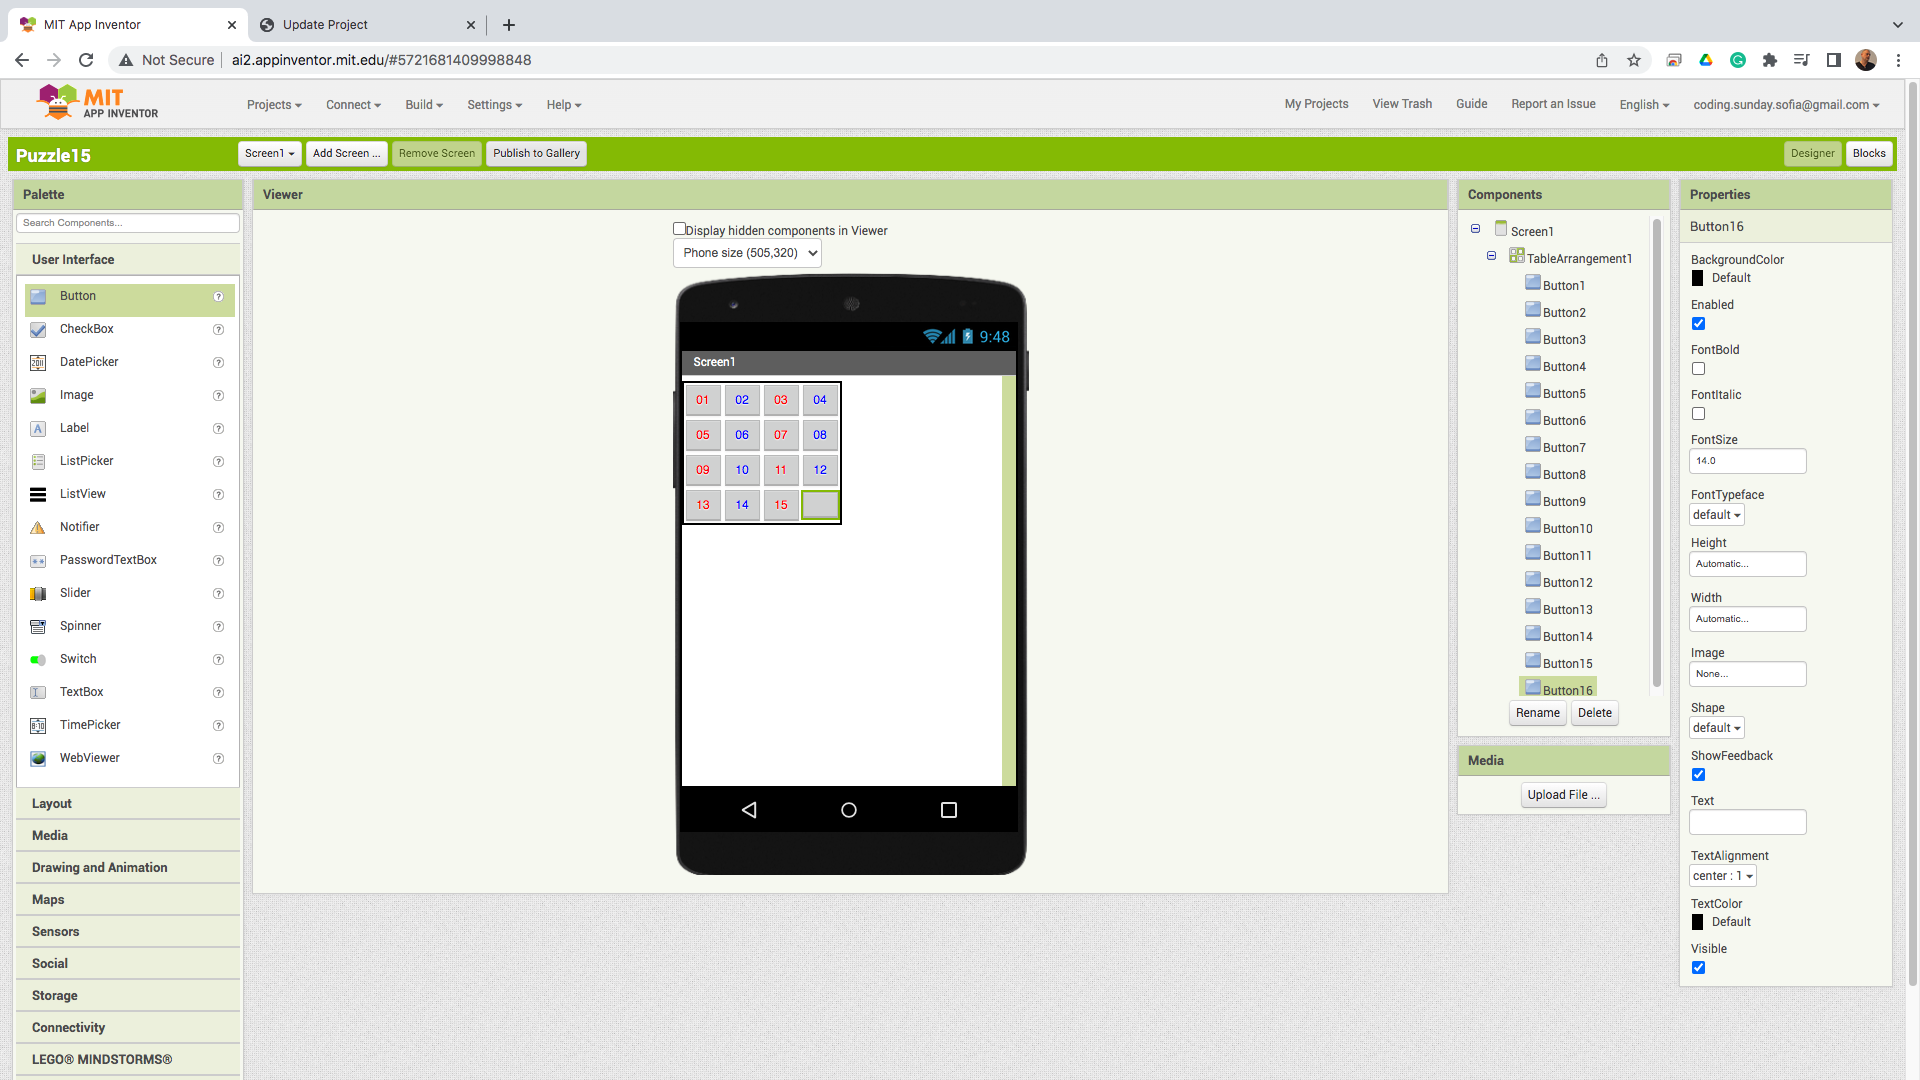
\includegraphics[width=1.0\linewidth,height=0.5\linewidth]{fig060021.png}
   \caption{Post to gallery button}
\label{fig060021}
\end{figure}

Even a simple description (Fig. \ref{fig060022}) of the application is important to users, as it is the second thing that catches their attention.

\begin{figure}[H]
   \centering
   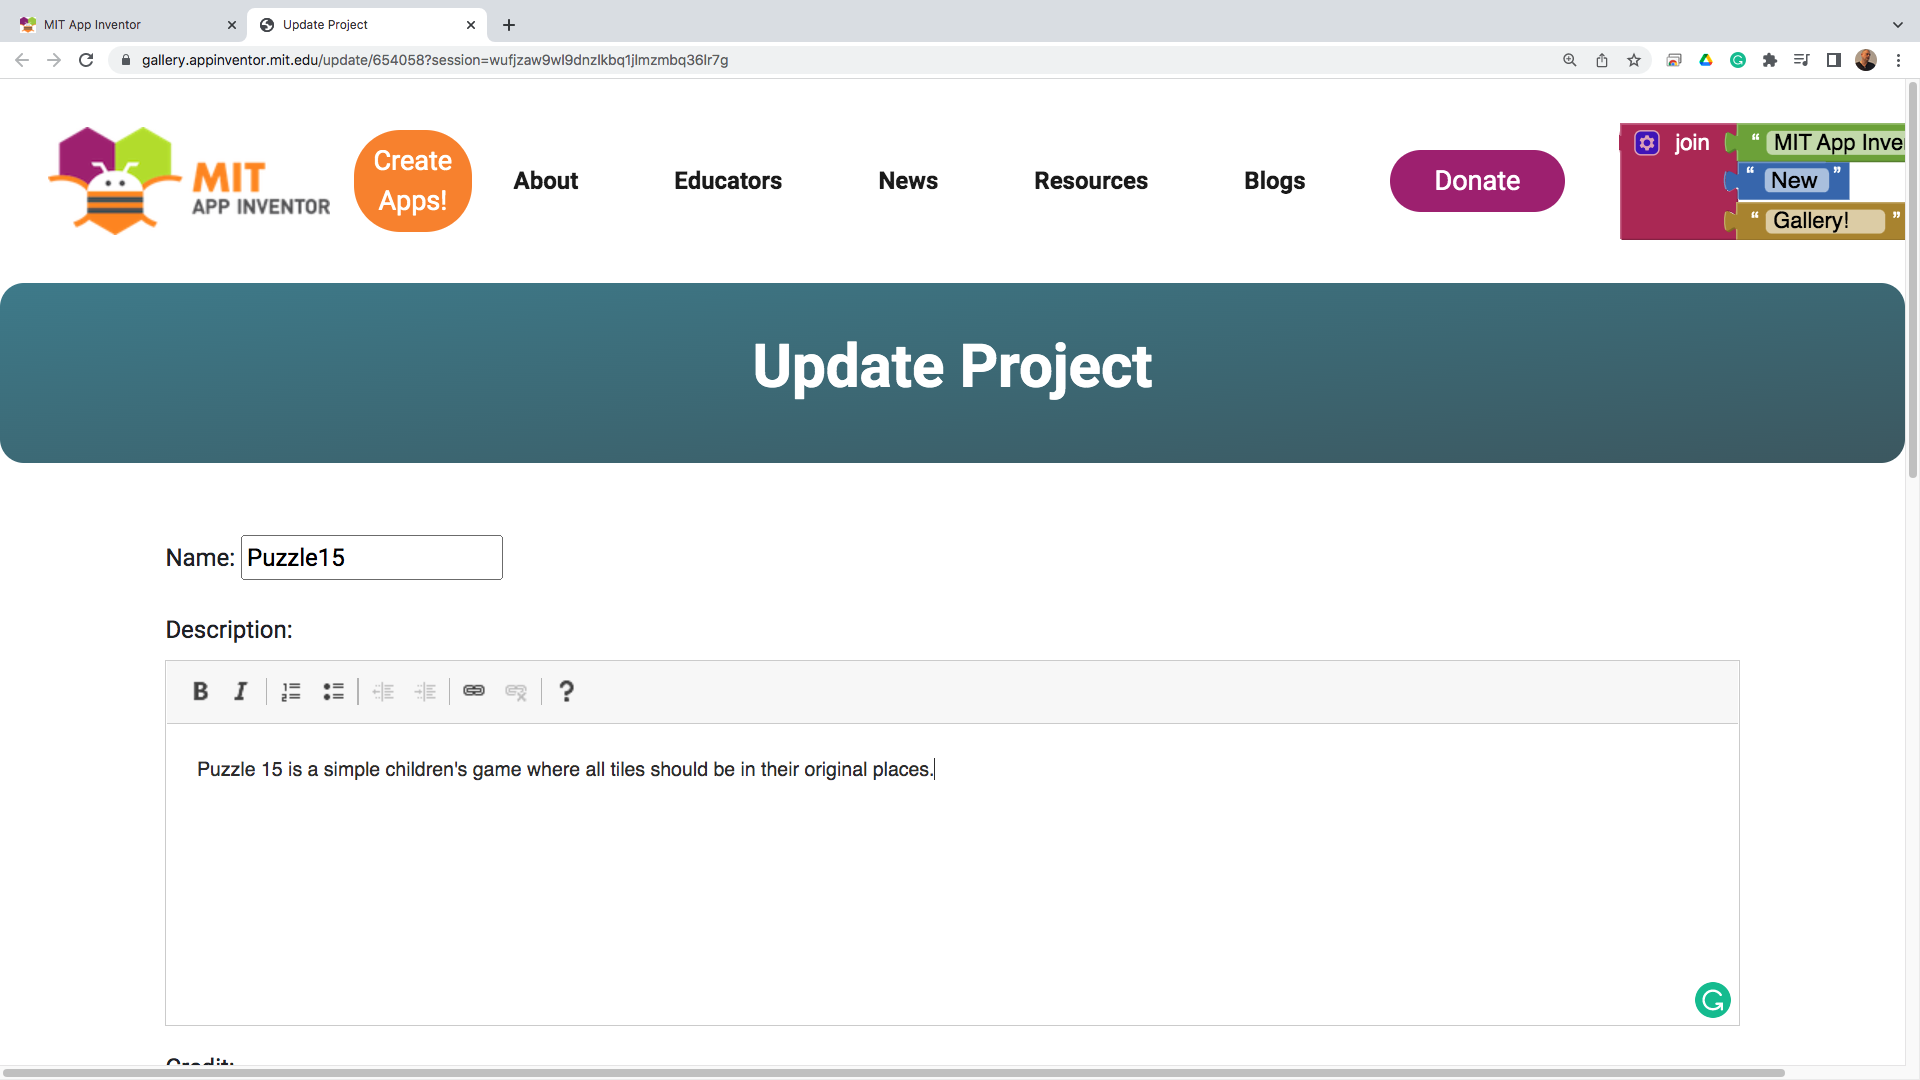
\includegraphics[width=1.0\linewidth,height=0.5\linewidth]{fig060022.png}
   \caption{Application Description}
\label{fig060022}
\end{figure}

The first most important thing in a software application is a picture, which can most attract the attention of users (Fig. \ref{fig060023}).

\begin{figure}[H]
   \centering
   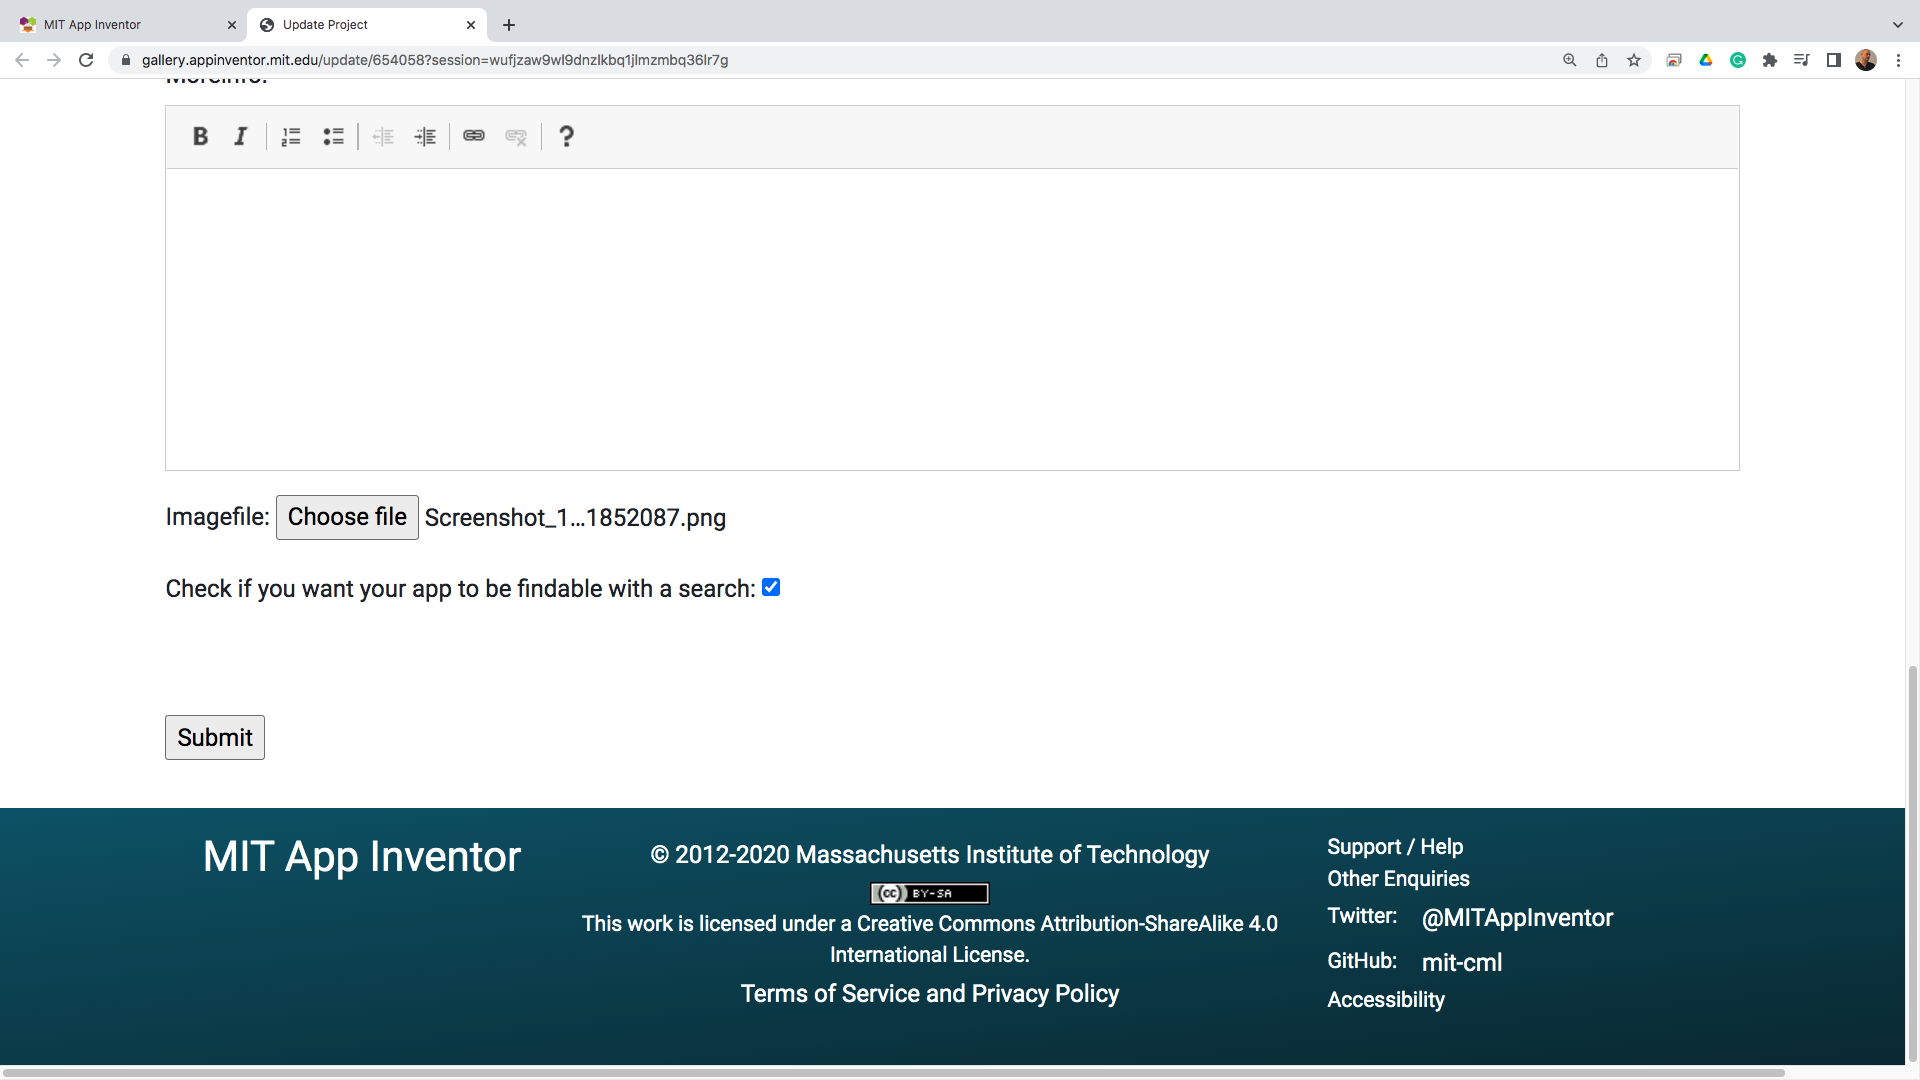
\includegraphics[width=1.0\linewidth,height=0.5\linewidth]{fig060023.png}
   \caption{Image to introduce the application}
\label{fig060023}
\end{figure}

On the project's public page (Fig. \ref{fig060024}), users can run the program or load it into the App Inventor environment.

\begin{figure}[H]
   \centering
   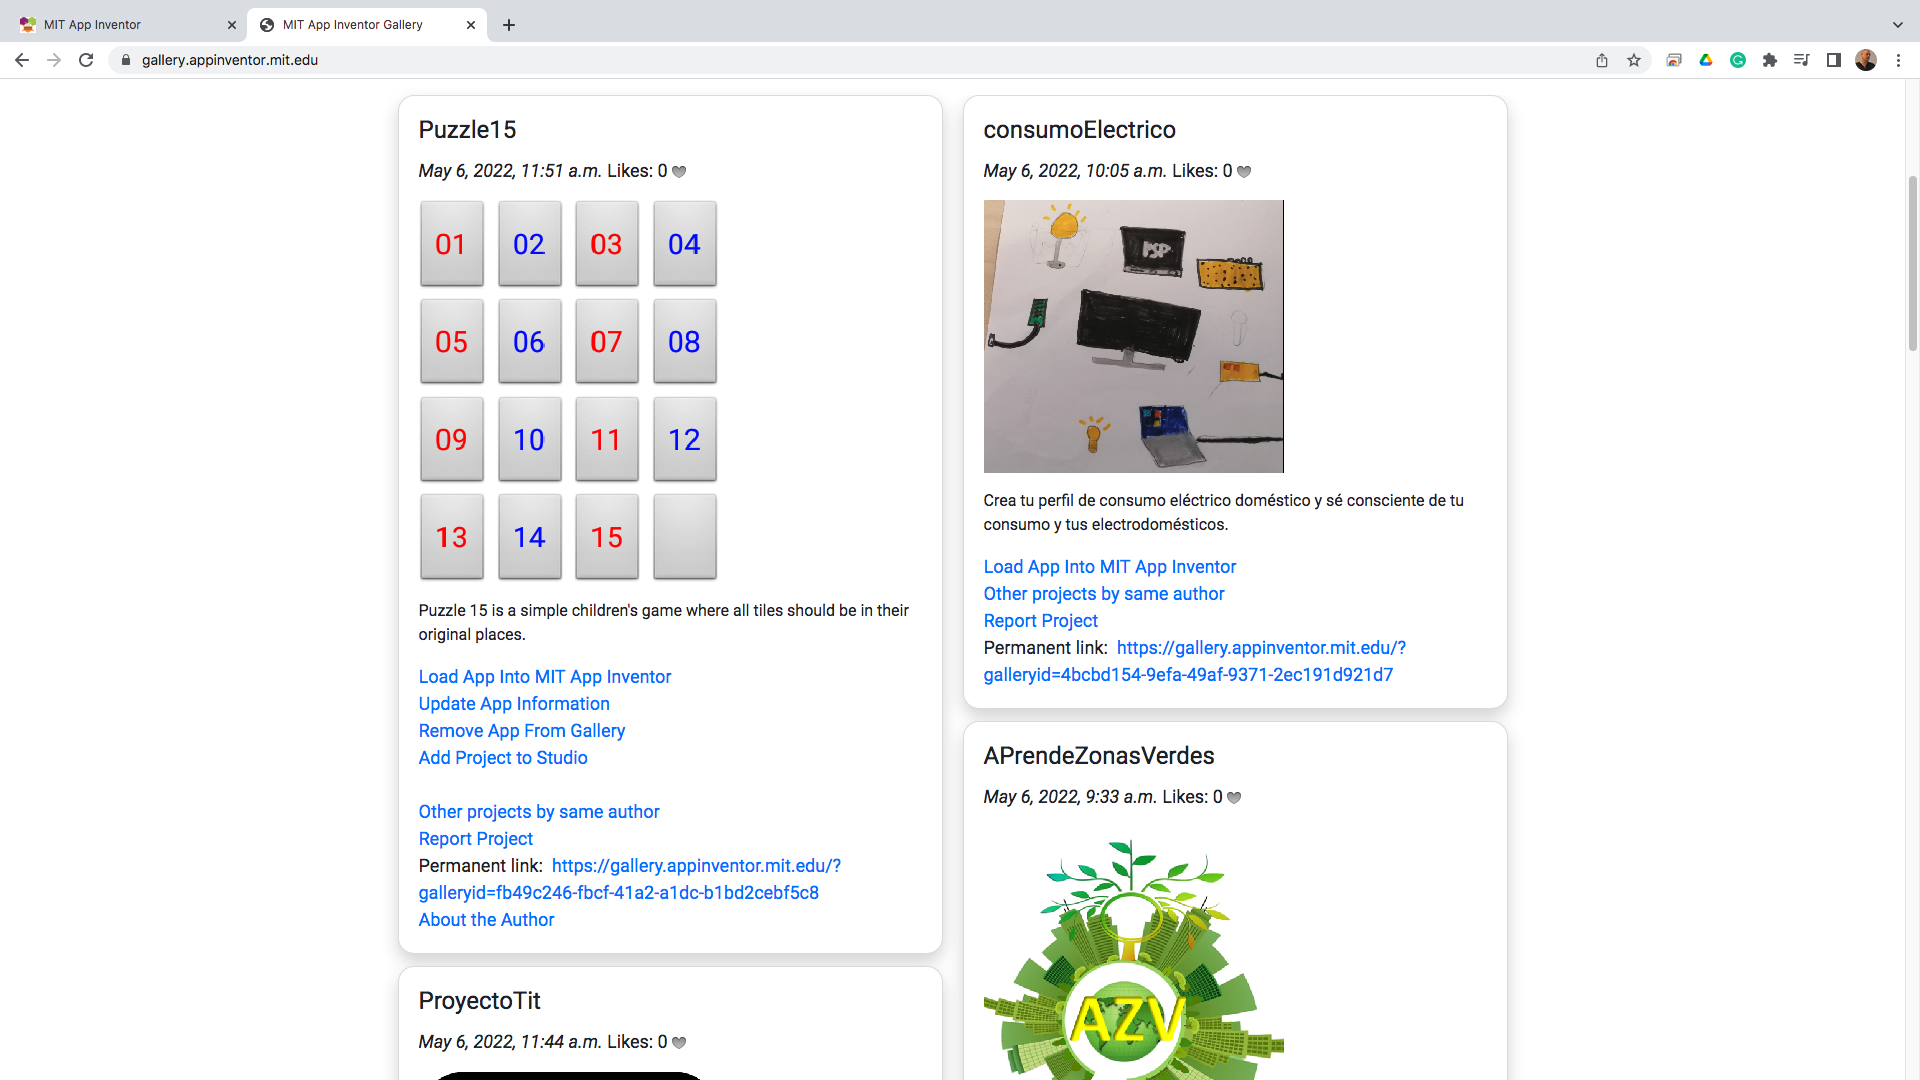
\includegraphics[width=1.0\linewidth,height=0.5\linewidth]{fig060024.png}
   \caption{Public project page}
\label{fig060024}
\end{figure}

The game is fully usable, but some functionality is still missing. It would be nice to add an option to auto-order the puzzle. The lack of supporting information is also a drawback. It is possible to add timekeeping to the arrangement, so that at a more advanced stage there is the possibility of organizing an online leaderboard. The listed functionalities carry a certain complexity and go beyond the scope of this presentation, but they are an ideal opportunity for additional exercise for the readers.
